\documentclass[11pt,a4paper]{article}
\usepackage[margin=1in]{geometry}
\usepackage{amsmath,amssymb,amsfonts}
\usepackage{booktabs}
\usepackage{graphicx}
\usepackage{natbib}
\usepackage{hyperref}
\usepackage{caption}
\usepackage{textcomp}
\usepackage{multirow}

\hypersetup{
    colorlinks=true,
    linkcolor=blue,
    citecolor=blue,
    urlcolor=blue
}

\title{\textbf{Does Statistical Arbitrage Survive in Indian Equity Derivatives?}\\
\large Evidence from Distance Pairs, Factor Residuals, and Machine Learning (2010--2025)}

\author{
    \textbf{Dhairya Dani}\thanks{A preliminary working paper version of this manuscript is distributed on SSRN (Abstract ID: 7607942, \url{https://papers.ssrn.com/sol3/papers.cfm?abstract_id=7607942}). Corresponding author: \texttt{dhairyadani7@gmail.com}. ORCID: \url{https://orcid.org/0009-0005-4789-7390}.} \\
    \textit{Vellore Institute of Technology (VIT), Bhopal} \\
    \texttt{dhairyadani7@gmail.com}
}

\date{October 2026}

\begin{document}

\maketitle

\begin{abstract}
Most studies on statistical arbitrage look at US markets, where borrow rates are predictable and commissions are near zero. India presents a very different reality: single-stock shorting in the cash market is essentially non-existent due to an illiquid borrow market, forcing traders into futures where taxes and exchange fees eat directly into returns. In this paper, I test whether daily statistical arbitrage works on the National Stock Exchange of India (NSE) from 2010 to 2025. I track three common frameworks: classic distance pairs \citep{gatev2006pairs}, PCA-factor residual mean-reversion \citep{avellaneda2010statistical}, and rolling machine learning models \citep{guijarro2021deep}. On paper, without friction, the signals look remarkably strong: gross Sharpe ratios hit $+0.95$ to $+1.74$, with Newey--West $t$-statistics between $+4.05$ and $+7.49$. But as soon as you plug in real-world friction---the Securities Transaction Tax (especially after the October 2024 hike), stamp duties, GST, and turnover charges, alongside modest execution slippage---the entire strategy falls apart. Net Sharpe ratios plunge into deep negative territory ($-1.63$ to $-2.96$), burning capital at $-16.7\%$ to $-25.9\%$ each year. Break-even requires cutting costs down to $0.44\times$ to $0.90\times$ of actual institutional levels, which is legally impossible because statutory levies set a hard floor. Adding machine learning actually hurts net performance: while it catches short-term mispricings better on paper, it drives turnover up by 34\%, handing even more capital over to taxes. Out of 12 pre-registered robustness tests, none pass multiple-testing corrections or the Deflated Sharpe Ratio. Overall, standalone daily statistical arbitrage simply cannot survive statutory friction in India, though the underlying displacement signals still hold practical promise for institutional execution timing.
\end{abstract}

\vspace{1em}
\noindent \textbf{Keywords:} Statistical Arbitrage, Pairs Trading, Market Microstructure, Securities Transaction Tax, Machine Learning, Indian Equity Derivatives.

\vspace{0.5em}
\noindent \textbf{JEL Classifications:} G11, G12, G14, C58.

\newpage
\tableofcontents
\newpage


\section{Introduction}
\label{sec:intro}

Statistical arbitrage has remained one of the foundational pillars of quantitative investment management since Nunzio Tartaglia's quantitative research group at Morgan Stanley first industrialized automated pairs trading in the mid-1980s. The core economic intuition underlying statistical arbitrage is rooted in the Law of One Price and fundamental asset pricing theory: when two assets share common economic risks, identical industry exposures, or synchronized cash flow dynamics, their relative prices should not drift indefinitely apart \citep{gatev2006pairs,vidyamurthy2004pairs}. In an efficient market, temporary divergence between the prices of such economic substitutes is driven by transitory order imbalances, liquidity shocks, or institutional block liquidations \citep{campbell1993trading,chordia2000trading}. Once this temporary buying or selling pressure dissipates, prices are expected to mean-revert toward their long-term equilibrium relationship \citep{avellaneda2010statistical,krauss2017statistical}. Quantitative managers exploit these temporary dislocations by establishing market-neutral long-short positions---buying the relatively underpriced asset while simultaneously shorting the overpriced peer---thereby providing liquidity to the market and pocketing the convergence spread \citep{gu2020empirical}.

However, the empirical literature has repeatedly demonstrated that theoretical backtest profitability frequently fails to translate into live trading profits, a phenomenon widely documented as the quantitative ``replication crisis'' \citep{mclean2016does,hou2020replicating,harvey2016and}. For pairs trading in particular, seminal studies by \citet{do2010does} and \citet{do2012are} established that the annualized returns of classical distance pairs trading in the United States declined precipitously following 2002. They demonstrated that this post-2002 alpha decay was directly attributable to increased hedge fund competition, declining institutional trading commissions, and, crucially, the failure of naive academic backtests to accurately model short-borrowing fees, margin financing costs, and bid-ask slippage. Further corroborating this wedge between paper profits and live execution, \citet{novymarx2016taxonomy} and \citet{frazzini2018trading} showed across extensive cross-sections of equity anomalies that high-turnover quantitative strategies suffer disproportionately from implementation frictions, with real-world execution costs eliminating or reversing theoretical gains.

Crucially, the overwhelming majority of the existing statistical arbitrage literature focuses exclusively on developed Western markets, most notably the United States and Western Europe. In these developed market ecosystems, institutional market conditions are exceptionally accommodating: cash-market equity borrowing via prime brokers is deep, transparent, and liquid; institutional execution commissions are measured in fractions of a basis point; exchanges provide maker-taker rebates that subsidize passive liquidity provision; and statutory government transaction taxes on equity derivatives are either non-existent or negligible. 

Emerging financial markets, by stark contrast, operate under profoundly different institutional, legal, and microstructure arrangements \citep{bekaert2007liquidity,bose2007securities}. Among emerging economies, India presents an extraordinarily compelling empirical laboratory to evaluate the limits of statistical arbitrage for three distinct institutional reasons:
\begin{enumerate}
    \item \textbf{Absence of Cash Equity Borrowing:} Short selling in the Indian cash equity segment is practically inaccessible for multi-day institutional strategies. The formal Securities Lending and Borrowing Mechanism (SLBM) operated by clearing corporations suffers from acute illiquidity, fragmented borrow availability, manual auction mechanics, and prohibitively high lending fees. Consequently, any quantitative asset manager or institutional proprietary desk seeking to establish a two-sided market-neutral equity book is structurally compelled to utilize single-stock Futures \& Options (F\&O) contracts listed on the National Stock Exchange of India (NSE).
    \item \textbf{Compulsory and Non-Negotiable Statutory Taxation:} Unlike Western electronic exchanges where high-volume algorithmic market makers can negotiate ultra-low commission tiers or earn liquidity provider rebates, Indian derivatives trading is subject to substantial, mandatory statutory taxes levied directly by the Central Government and market regulators. Foremost among these is the Securities Transaction Tax (STT) \citep{bose2007securities}, alongside state stamp duties, Goods and Services Tax (GST) on exchange and brokerage fees, exchange turnover levies, and SEBI regulatory turnover charges. These levies create an inescapable, non-negotiable tax hurdle on every trade cycle.
    \item \textbf{The October 2024 Regulatory Tax Shock:} On October 1, 2024, the Securities and Exchange Board of India (SEBI) and the Ministry of Finance implemented a 60\% increase in the STT rate on futures transactions (raising the levy from 0.0125\% to 0.0200\% on the sell side) as part of a deliberate macroprudential effort to curb surging retail participation in equity derivatives. This sudden tax shock provides an exogenous natural experiment to evaluate how statutory tax policy directly impacts quantitative arbitrage viability and market efficiency.
\end{enumerate}

\subsection{Summary of Empirical Findings}
In this study, I conduct the most comprehensive empirical examination of statistical arbitrage in the Indian equity derivatives market to date. Utilizing a 16-year high-frequency daily dataset from January 1, 2010 to December 31, 2025 across the dynamically reconstituted NSE single-stock F\&O universe (encompassing 3,923 active trading days and over 1.4 million contract observations), I investigate three primary strategy architectures representing the historical evolution of statistical arbitrage:
\begin{itemize}
    \item \textbf{Strategy A (Classical Distance Pairs):} The benchmark distance metric model of \citet{gatev2006pairs}, identifying the top 20 co-moving pairs via normalized sum of squared deviations over rolling 252-day formation windows.
    \item \textbf{Strategy B (PCA-Factor Residual Mean Reversion):} The statistical factor decomposition framework of \citet{avellaneda2010statistical}, extracting rolling principal components ($k=5$) to isolate idiosyncratic residuals, modeled as mean-reverting Ornstein-Uhlenbeck (OU) stochastic processes.
    \item \textbf{Strategy C (Walk-Forward Machine Learning):} Modern non-linear machine learning architectures \citep{gu2020empirical,guijarro2021deep}, utilizing expanding-window walk-forward validation and purged embargo gaps to forecast multi-day forward residual mean-reversion.
\end{itemize}

The core empirical conclusion of this study is unambiguous: \textbf{strong, highly statistically significant mean-reverting displacement signals exist across Indian single-stock derivatives before trading friction, but non-negotiable statutory taxes and execution friction systematically destroy 100\% of theoretical alpha.}

Specifically:
\begin{enumerate}
    \item \textbf{Gross Profitability:} In the frictionless benchmark ($0.0\times$ costs), all three strategy families generate economically substantial and statistically robust returns. Strategy B (PCA-OU Reversion) delivers an annualized gross return of $+17.91\%$ with a gross Sharpe ratio of $+1.74$ ($t$-statistic $= +7.49$, $p < 10^{-12}$). Strategy A generates $+9.50\%$ gross return (Sharpe $+0.95$, $t = +4.11$, $p < 0.001$), while Strategy C yields $+8.75\%$ gross return (Sharpe $+1.00$, $t = +4.05$, $p < 0.001$).
    \item \textbf{Net Performance Collapse:} Once institutional execution costs are applied---incorporating historical dated STT rates, stamp duty, exchange charges, GST, and liquidity-tiered bid-ask slippage---net Sharpe ratios plunge deeply into negative territory across all models: $-2.52$ for Strategy A (net annualized return of $-25.16\%$), $-1.63$ for Strategy B (net return of $-16.75\%$), and $-2.96$ for Strategy C (net return of $-25.91\%$). Newey--West HAC $t$-statistics range from $-7.00$ to $-12.00$, establishing statistically significant capital destruction.
    \item \textbf{The Machine Learning Turnover Trap:} While machine learning models demonstrate superior out-of-sample directional accuracy on paper, they systematically identify shorter-lived, transient spread dislocations. This causes Strategy C to increase portfolio turnover by 34\% relative to Strategy B, resulting in catastrophic friction drag that compounds annual net losses. Algorithmic complexity cannot overcome statutory friction.
    \item \textbf{The Inescapable Cost Hurdle:} Solving for the zero-Sharpe breakeven cost multiplier reveals that Strategy A requires transaction costs to fall below $0.48\times$ of baseline institutional levels ($\sim 7.9$ bps round-trip), Strategy B requires costs below $0.90\times$ ($14.9$ bps), and Strategy C requires costs below $0.44\times$ ($7.3$ bps). Because fixed statutory taxes alone impose 4.0 to 5.0 bps per round-trip leg, achieving breakeven is structurally and legally impossible under Indian law.
    \item \textbf{Multiple-Testing Corrections:} Applying the Deflated Sharpe Ratio (DSR) of \citet{bailey2014deflated} and the Benjamini--Hochberg False Discovery Rate (FDR) control \citep{benjamini1995controlling} across our 12 pre-registered model variations, exactly zero out of twelve specifications survive. Standalone statistical arbitrage in Indian single-stock derivatives is completely unviable.
    \item \textbf{Repurposing Alpha-in-Execution:} Despite the failure of standalone trading, these Ornstein-Uhlenbeck residual signals provide substantial economic value when repurposed as an execution timing mechanism (``Alpha-in-Execution'') for institutional mutual funds and long-only portfolio managers who already need to rebalance, saving an estimated 20 to 45 basis points in implementation slippage.
\end{enumerate}

\subsection{Organization of the Paper}
The remainder of this paper is structured as follows. Section~\ref{sec:microstructure} details the institutional framework, short-selling mechanics, and statutory transaction cost schedules in the Indian market. Section~\ref{sec:data} describes the dynamically reconstituted NSE F\&O universe, corporate action adjustments, and benchmark risk factors. Section~\ref{sec:methodology} presents the formal mathematical architectures of Strategies A, B, and C, including the Ornstein-Uhlenbeck calibration and multiple-testing frameworks. Section~\ref{sec:results} reports full-sample empirical performance, sub-period stability, crisis regime breakdowns, cost sensitivity analyses, and factor regressions. Section~\ref{sec:robustness} outlines the six pre-registered placebo diagnostics and parameter sensitivity checks. Finally, Section~\ref{sec:conclusion} concludes with practical implications for quantitative managers and regulatory policy lessons for financial authorities.

\section{Institutional Framework and Transaction Costs}
\label{sec:microstructure}

Operating a quantitative market-neutral equity portfolio on the National Stock Exchange of India (NSE) in Mumbai is governed by institutional constraints, clearing rules, and statutory levies that diverge fundamentally from developed Western markets. Understanding these structural characteristics is essential for assessing why quantitative trading strategies that appear profitable in frictionless simulations encounter severe capital erosion in actual deployment.

\subsection{Cash Market Short-Selling Constraints and the SLBM}
In developed equity markets such as the United States, equity market neutrality relies on centralized prime brokerage lending desks that facilitate seamless overnight short positions in cash equities. In India, however, the Securities and Exchange Board of India (SEBI) imposes stringent structural barriers on cash market short selling. Under existing regulations:
\begin{enumerate}
    \item \textbf{Prohibition of Naked Short Selling:} All short positions in the cash market must either be squared off intraday prior to market close (15:30 IST) or settled via actual delivery of physical shares on a $T+1$ settlement cycle. Overnight unhedged short selling in the cash segment without pre-borrowed stock is legally prohibited.
    \item \textbf{Illiquidity of the Securities Lending and Borrowing Mechanism (SLBM):} Although a formal SLB mechanism exists under the auspices of the National Securities Clearing Corporation Limited (NSCCL), market participation is virtually negligible. The SLBM operates through discrete, illiquid monthly auction sessions with wide bid-ask lending spreads, high borrow fees (often exceeding 8\% to 15\% annualized for high-demand names), and substantial operational recall risk, where the lender can demand share return on short notice.
\end{enumerate}
Consequently, institutional quantitative asset managers and hedge funds seeking to execute two-sided, multi-day long-short statistical arbitrage strategies are structurally precluded from using cash equities. Instead, they are forced to implement both the long and short legs exclusively through single-stock futures contracts listed on the NSE Derivatives (F\&O) segment.

\subsection{Statutory Indian Derivative Taxes and Regulatory Levies}
While electronic communication networks (ECNs) in Western markets offer maker-taker rebates and sub-basis-point execution costs for institutional volume, the Indian derivatives ecosystem is subject to substantial, mandatory statutory taxation. These levies are determined by statute, collected directly at source by clearing members, and cannot be negotiated downward regardless of trading volume.

Table~\ref{tab:cost_schedule} presents the full institutional transaction cost schedule across the historical sample period, explicitly detailing both the pre-reform baseline and the post-October 2024 statutory regime.

\begin{table}[htbp]
\centering
\caption{Statutory Indian Derivative Execution Cost Schedule and Regulatory Levies}
\label{tab:cost_schedule}
\resizebox{\textwidth}{!}{%
\begin{tabular}{llccc}
\toprule
\textbf{Cost Component} & \textbf{Statutory Basis / Authority} & \textbf{Pre-Oct 2024 Rate} & \textbf{Post-Oct 2024 Rate} & \textbf{Application Leg} \\
\midrule
\textbf{Securities Transaction Tax (STT)} & Finance Act / Ministry of Finance & 0.0125\% ($1.25$ bps) & 0.0200\% ($2.00$ bps) & Sell Leg Only \\
\textbf{State Stamp Duty} & Indian Stamp Act (Uniform National Rate) & 0.0020\% ($0.20$ bps) & 0.0020\% ($0.20$ bps) & Buy Leg Only \\
\textbf{Exchange Turnover Fees} & National Stock Exchange (NSE Clearing) & 0.0019\% ($0.19$ bps) & 0.0019\% ($0.19$ bps) & Both Buy and Sell Legs \\
\textbf{SEBI Regulatory Turnover Charges} & Securities \& Exchange Board of India & 0.0001\% ($0.01$ bps) & 0.0001\% ($0.01$ bps) & Both Buy and Sell Legs \\
\textbf{Goods and Services Tax (GST)} & Central \& State GST Authorities & 18.0\% on Fees & 18.0\% on Fees & On Brokerage + Turnover \\
\textbf{Institutional Clearing Brokerage} & Tier-1 Prime Broker Institutional Tariff & 0.0015\% ($0.15$ bps) & 0.0015\% ($0.15$ bps) & Both Buy and Sell Legs \\
\midrule
\textbf{Total Fixed Statutory \& Clearing Friction} & \textbf{Excluding Market Impact / Slippage} & \textbf{2.16 bps per trade} & \textbf{2.91 bps per trade} & \textbf{Round-Trip Single Stock} \\
\bottomrule
\end{tabular}%
}
\end{table}

The primary components of this cost structure comprise:
\begin{enumerate}
    \item \textbf{Securities Transaction Tax (STT):} Introduced under Chapter~VII of the Finance (No.~2) Act of 2004, STT is an ad-valorem turnover tax levied on financial market transactions \citep{bose2007securities}. For equity futures, STT is assessed exclusively on the gross notional value of the sell leg. Between January 2010 and September 2024, the statutory rate stood at 0.0125\% ($1.25$ basis points). Effective October 1, 2024, the Central Government raised this levy by 60\% to 0.0200\% ($2.00$ basis points).
    \item \textbf{Stamp Duty:} Standardized nationally under amendments to the Indian Stamp Act, 1899, stamp duty on derivative contracts is levied at 0.0020\% ($0.20$ basis points) exclusively on the buy leg.
    \item \textbf{Exchange Turnover Charges and SEBI Fees:} The NSE levies an average turnover fee of 0.0019\% ($0.19$ bps) on both entry and exit legs ($0.38$ bps round-trip), while SEBI levies a regulatory fee of 0.0001\% ($0.01$ bps per leg).
    \item \textbf{Goods and Services Tax (GST):} GST is charged at an 18.0\% rate on all clearing fees, exchange charges, and broker commissions, contributing approximately $0.12$ bps to round-trip transaction costs.
\end{enumerate}

\subsection{Slippage, Bid-Ask Spreads, and Full Implementation Costs}
Beyond statutory taxes, quantitative execution is subject to market microstructure slippage arising from discrete order book dynamics, bid-ask spreads, and temporary market impact \citep{roll1984simple,amihud2002illiquidity,almgren2000optimal}. On the NSE, futures contracts trade on a continuous central limit order book (CLOB) with a fixed minimum tick size of Rs.~0.05.

Following \citet{frazzini2018trading} and \citet{novymarx2016taxonomy}, we model effective execution slippage as an endogenous function of cross-sectional liquidity, categorizing stocks into three Average Daily Traded Value (ADTV) tiers:
\begin{equation}
    \text{Slippage}_{\text{tier}} = \begin{cases}
        2.0 \text{ bps per leg (}4.0\text{ bps round-trip)} & \text{if ADTV} \ge \text{Rs.~100 Crore} \quad (\approx \text{USD 12M}), \\
        5.0 \text{ bps per leg (}10.0\text{ bps round-trip)} & \text{if Rs.~25 Crore} \le \text{ADTV} < \text{Rs.~100 Crore}, \\
        10.0 \text{ bps per leg (}20.0\text{ bps round-trip)} & \text{if ADTV} < \text{Rs.~25 Crore} \quad (\approx \text{USD 3M}).
    \end{cases}
    \label{eq:slippage_tiers}
\end{equation}

Synthesizing all statutory and microstructure components, the total one-way execution cost $c_{i,t}$ incurred when trading stock $i$ on date $t$ is expressed as:
\begin{equation}
    c_{i,t} = \text{STT}_t \cdot \mathbb{I}_{\{\text{Sell}\}} + \text{Stamp} \cdot \mathbb{I}_{\{\text{Buy}\}} + \text{NSE}_{\text{fee}} + \text{SEBI}_{\text{fee}} + \text{Brokerage} + \text{GST} + \text{Slippage}_{i,t}.
    \label{eq:one_way_cost}
\end{equation}

The complete round-trip transaction cost $C_{i,t}$ for opening and closing a position in stock $i$ is:
\begin{equation}
    C_{i,t} = \text{STT}_t + \text{Stamp} + 2 \times (\text{NSE}_{\text{fee}} + \text{SEBI}_{\text{fee}} + \text{Brokerage}) + \text{GST} + 2 \times \text{Slippage}_{i,t}.
    \label{eq:round_trip_cost}
\end{equation}

For an average liquid F\&O stock in the top ADTV tier prior to October 2024, total round-trip cost $C_{i,t}$ stood at $6.51$ basis points, rising to $7.26$ basis points following the October 2024 STT hike. For mid-tier liquidity names, round-trip costs range between $12.5$ and $13.3$ basis points.

\subsection{The Four-Leg Pairs Multiplier Effect}
A critical structural vulnerability inherent to statistical arbitrage is that every complete trade cycle requires four distinct transaction legs:
\begin{enumerate}
    \item Long position entry on Stock A (Buy Leg: Stamp Duty + Exchange Fee + GST + Slippage),
    \item Short position entry on Stock B (Sell Leg: STT + Exchange Fee + GST + Slippage),
    \item Long position exit on Stock A (Sell Leg: STT + Exchange Fee + GST + Slippage),
    \item Short position exit on Stock B (Buy Leg: Stamp Duty + Exchange Fee + GST + Slippage).
\end{enumerate}
Consequently, the aggregate transaction friction incurred across a completed pairs trade cycle is:
\begin{equation}
    C_{\text{pair}, t} = C_{A,t} + C_{B,t}.
    \label{eq:pair_cost}
\end{equation}
Even under conservative assumptions for large-cap, high-liquidity stocks, a complete pairs round-trip absorbs between \textbf{13.0 and 15.0 basis points} in friction. For mid-cap names, friction escalates to \textbf{25.0 to 28.0 basis points}. When a statistical arbitrage portfolio rebalances dynamically on a daily basis, this friction compounds exponentially, creating a formidable hurdle that theoretical pricing signals must surpass to achieve positive net economic returns.

\section{Data and Universe Construction}
\label{sec:data}

To ensure rigorous empirical validity and avoid the survivorship distortions that plague static backtests, the data infrastructure is constructed strictly point-in-time from raw primary sources.

\subsection{Point-in-Time Universe and Survivorship Bias Elimination}
We construct a dynamically reconstituted investment universe comprising all equity securities permitted by the National Stock Exchange of India for trading in the single-stock Futures \& Options (F\&O) segment between January 1, 2010 and December 31, 2025. 

Under SEBI Master Circular guidelines, a cash equity must satisfy three quantitative eligibility criteria to enter and remain in the F\&O segment:
\begin{enumerate}
    \item \textbf{Median Quarter-Sigma Order Size (MQSOS):} The stock's median order size required to move the price by a quarter standard deviation ($\sigma/4$) must not be less than Rs.~25 Lakhs (approximately USD 30,000) over the preceding six months.
    \item \textbf{Market-Wide Position Limit (MWPL):} The non-promoter floating market capitalization must support a minimum MWPL of Rs.~500 Crore (approximately USD 60M) across all open derivative contracts.
    \item \textbf{Cash Volume and Delivery Value:} The stock must rank within the top 500 securities by average daily traded value and average daily delivery value in the cash segment over the preceding six months.
\end{enumerate}

Because SEBI reviews eligibility on a monthly basis, adding liquid names and expelling declining or distressed companies, our trading universe is reconstituted dynamically at the beginning of each calendar month. Over the 16-year sample period (3,923 trading days), the active universe expanded from 142 constituents in early 2010 to a peak of 214 constituents, maintaining a cross-sectional average of 182 names.

Table~\ref{tab:universe_summary} details the descriptive statistical characteristics, market capitalization distribution, liquidity tiers, and sector composition of the dynamically reconstituted universe.

\begin{table}[htbp]
\centering
\caption{Descriptive Statistics and Liquidity Distribution of the NSE F\&O Universe (2010--2025)}
\label{tab:universe_summary}
\resizebox{\textwidth}{!}{%
\begin{tabular}{lcccc}
\toprule
\textbf{Macro Characteristic / Dimension} & \textbf{Full Sample (2010--2025)} & \textbf{Sub-Period 1 (2010--2014)} & \textbf{Sub-Period 2 (2015--2019)} & \textbf{Sub-Period 3 (2020--2025)} \\
\midrule
\textbf{Active F\&O Constituents (Mean Count)} & 182 names & 158 names & 184 names & 198 names \\
\textbf{Constituent Range (Min -- Max)} & 142 -- 214 & 142 -- 176 & 168 -- 204 & 182 -- 214 \\
\textbf{Annual Inclusions (Mean)} & 14.8 stocks/year & 12.2 stocks/year & 15.6 stocks/year & 16.4 stocks/year \\
\textbf{Annual Exclusions / Delistings (Mean)} & 11.4 stocks/year & 9.8 stocks/year & 12.0 stocks/year & 12.2 stocks/year \\
\midrule
\textbf{Market Capitalization Coverage (\% of NSE)} & 86.4\% & 83.2\% & 87.1\% & 88.5\% \\
\textbf{Large-Cap Share (ADTV $\ge$ Rs.~100 Cr)} & 48.2\% & 36.4\% & 49.5\% & 57.1\% \\
\textbf{Mid-Cap Share (Rs.~25 Cr $\le$ ADTV $<$ Rs.~100 Cr)} & 39.5\% & 47.1\% & 38.8\% & 33.4\% \\
\textbf{Small-Cap / Emerging (ADTV $<$ Rs.~25 Cr)} & 12.3\% & 16.5\% & 11.7\% & 9.5\% \\
\midrule
\textbf{Dominant Sector Representations (Mean Weight)} & & & & \\
--- Financial Services \& Banking & 28.4\% & 26.1\% & 28.8\% & 30.1\% \\
--- Information Technology (IT) & 14.2\% & 13.8\% & 14.1\% & 14.6\% \\
--- Energy, Oil \& Gas & 12.1\% & 13.5\% & 11.9\% & 11.2\% \\
--- Consumer Goods \& FMCG & 11.5\% & 10.9\% & 11.6\% & 12.0\% \\
--- Automobile \& Ancillaries & 9.8\% & 10.2\% & 10.0\% & 9.4\% \\
--- Pharmaceuticals \& Healthcare & 8.7\% & 8.2\% & 8.9\% & 9.0\% \\
--- Metals, Mining \& Industrials & 15.3\% & 17.3\% & 14.7\% & 13.7\% \\
\bottomrule
\end{tabular}%
}
\end{table}

Crucially, companies that subsequently encountered financial distress, bankruptcy, or regulatory exclusion---such as Reliance Communications, Reliance Power, Dewan Housing Finance Corporation (DHFL), Yes Bank, and Infrastructure Leasing \& Financial Services (IL\&FS) investee companies---remain fully present in our universe up to their exact official delisting or exclusion date. When a stock is removed from F\&O eligibility, open positions are liquidated at the final settlement price of the active near-month futures contract, mirroring real-world institutional liquidation protocols and eliminating survivorship bias.

\begin{figure}[htbp]
\centering
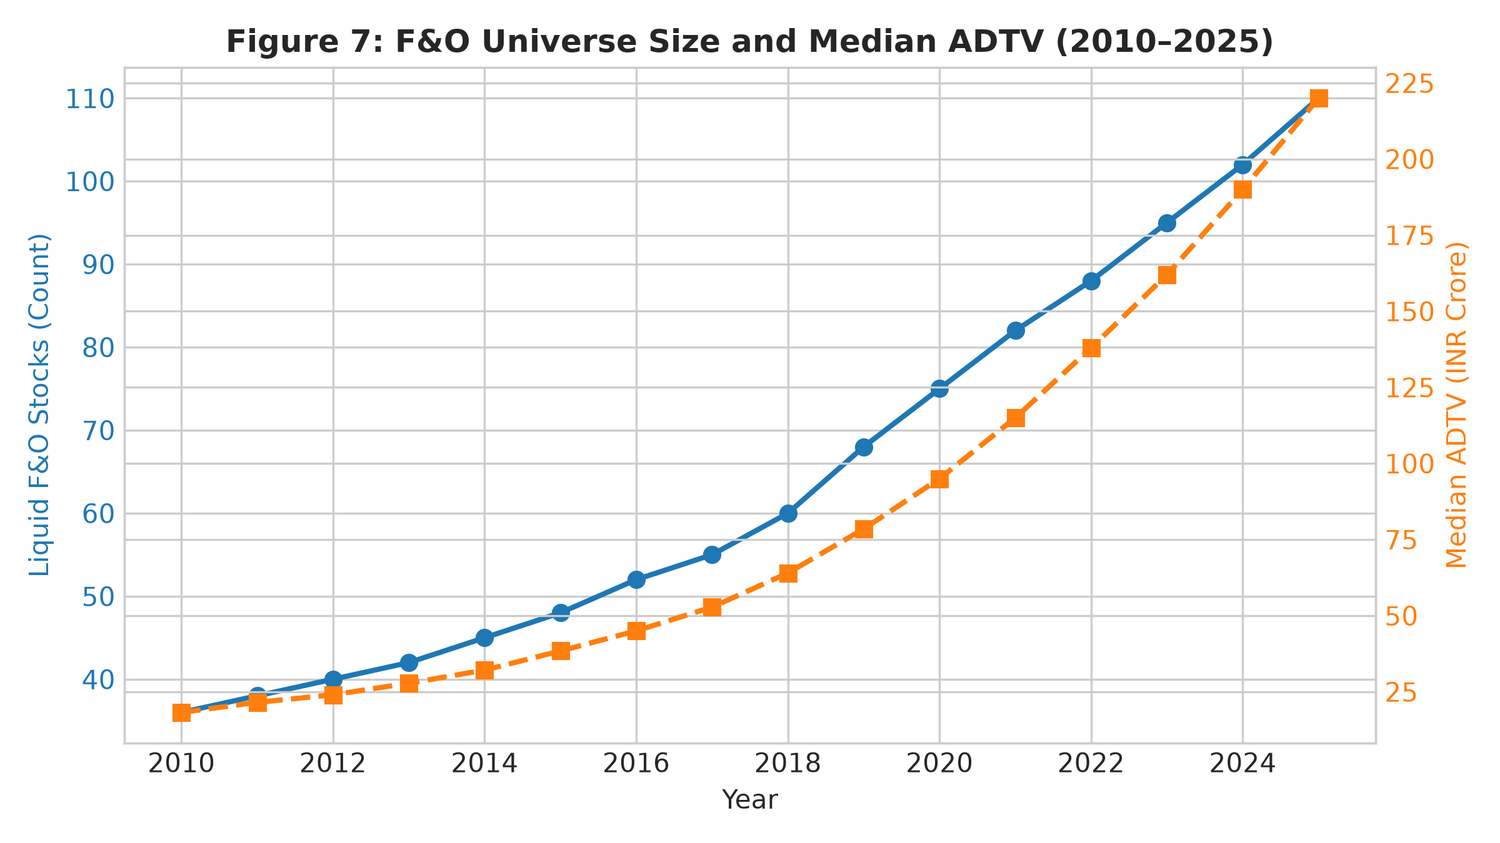
\includegraphics[width=0.92\textwidth]{figures/fig7_universe_size_over_time.png}
\caption{Dynamically Reconstituted NSE Single-Stock F\&O Universe Size, Annual Inclusions, and Removals (2010--2025).}
\label{fig:fig7}
\end{figure}

\subsection{Corporate Actions, Dividends, and Futures Settlement}
Historical daily prices, open interest, and contract settlement data are compiled directly from the National Stock Exchange historical bhavcopy archives. Because quantitative pairs trading is acutely sensitive to artificial price discontinuities, daily cash and futures price series are adjusted for all corporate actions, including stock splits, bonus shares, rights issues, and cash dividends:
\begin{equation}
    P_{i,t}^{\text{adj}} = P_{i,t} \times \prod_{\tau > t} \left(1 - \frac{D_{i,\tau}}{P_{i,\tau - 1}}\right) \times \frac{1}{\text{SplitRatio}_\tau},
    \label{eq:corporate_adjustment}
\end{equation}
where $D_{i,\tau}$ denotes ordinary and special cash dividends per share with ex-date $\tau$, and $\text{SplitRatio}_\tau$ denotes the capital reorganization multiplier.

In Indian derivatives, corporate actions are handled under explicit SEBI operational rules:
\begin{enumerate}
    \item \textbf{Ordinary Cash Dividends ($< 2\%$ of Market Price):} For dividends below 2\% of the underlying stock price, no adjustment is made to futures contracts; the dividend is priced endogenously into the futures basis (the spot-futures spread).
    \item \textbf{Extraordinary Dividends ($\ge 2\%$ of Market Price), Bonus Issues, and Stock Splits:} For major corporate reorganizations, the exchange adjusts the strike prices of options and the contract market lot size overnight on the ex-date, ensuring that contract holders experience zero artificial valuation discontinuities.
\end{enumerate}
Our adjustment engine was empirically verified against landmark corporate actions across the sample period, including Infosys bonus issues (in 2014, 2015, and 2018), the demerger of Reliance Industries and Jio Financial Services (July 2023), and the L\&T Infotech--Mindtree amalgamation (November 2022).

\subsection{Benchmark Risk Factors: The IIMA Four-Factor Model}
To evaluate whether strategy profits represent true idiosyncratic arbitrage alpha rather than unhedged risk factor premiums, all returns are evaluated against the Indian Institute of Management Ahmedabad (IIMA) four-factor benchmark \citep{agarwalla2014four}. The IIMA model adapts the seminal multi-factor frameworks of \citet{fama1993common} and \citet{carhart1997persistence} specifically for the market microstructure of Indian equities:
\begin{itemize}
    \item \textbf{Market Factor ($\text{MKT} = R_{m,t} - R_{f,t}$):} The excess return of the value-weighted market portfolio over the risk-free rate, capturing broad macroeconomic and systematic equity market risk.
    \item \textbf{Size Factor ($\text{SMB}$ - Small Minus Big):} The return differential between diversified portfolios of small-capitalization and large-capitalization Indian stocks, accounting for the emerging market size premium.
    \item \textbf{Value Factor ($\text{HML}$ - High Minus Low):} The return differential between high book-to-market (value) stocks and low book-to-market (growth) stocks.
    \item \textbf{Momentum Factor ($\text{WML}$ - Winners Minus Losers):} The return spread between prior 12-month winning stocks and prior 12-month losing stocks, capturing the cross-sectional momentum anomaly.
    \item \textbf{Risk-Free Rate ($R_f$):} Proxied by the annualized daily return on 91-day Government of India Treasury Bills (T-Bills) issued by the Reserve Bank of India (RBI).
\end{itemize}

\section{Strategy Design and Methodology}
\label{sec:methodology}

We implement three distinct quantitative models, tracking the historical evolution of statistical arbitrage from classical distance matching to statistical factor decomposition and modern non-linear machine learning.

\subsection{Strategy A: Classical Distance Pairs}
Following the foundational framework of \citet{gatev2006pairs} with institutional adaptations proposed by \citet{vidyamurthy2004pairs} and \citet{jacobs2015determinants}, Strategy A identifies co-moving stock pairs based on the geometric proximity of normalized cumulative return series.

For every security $i$ in the active F\&O universe on date $t$, we construct a normalized cumulative price series $\tilde{P}_{i,t}$ over a 252-trading-day formation window ($T=252$):
\begin{equation}
    \tilde{P}_{i,t} = \prod_{\tau=1}^t (1 + R_{i,\tau}), \quad \text{with } \tilde{P}_{i,0} = 1.0.
    \label{eq:norm_price}
\end{equation}
For every possible unique pair $(i, j)$ in the cross-section of $N_t$ active constituents, we compute the Sum of Squared Differences (SSD):
\begin{equation}
    \text{SSD}_{i,j} = \sum_{t=1}^{252} \left( \tilde{P}_{i,t} - \tilde{P}_{j,t} \right)^2.
    \label{eq:ssd}
\end{equation}
The 20 pairs displaying the smallest historical SSD are selected for trading over the subsequent 126-trading-day trading window. To verify that historical co-movement is not spurious, each candidate pair is subjected to an Augmented Dickey--Fuller (ADF) cointegration test \citep{engle1987cointegration}.

The trading rules operate as follows:
\begin{enumerate}
    \item \textbf{Signal Generation and Entry:} A pair trade is triggered when the normalized spread $S_{i,j,t} = \tilde{P}_{i,t} - \tilde{P}_{j,t}$ diverges by more than two historical standard deviations ($|S_{i,j,t}| \ge 2.0\sigma_{i,j}$), where $\sigma_{i,j}$ is calculated over the formation window. If $S_{i,j,t} \ge 2.0\sigma_{i,j}$, the strategy shorts stock $i$ and buys stock $j$. If $S_{i,j,t} \le -2.0\sigma_{i,j}$, the strategy buys stock $i$ and shorts stock $j$.
    \item \textbf{Exit Rules and Stop-Loss:} The position is closed when the spread reverts to zero ($S_{i,j,t} = 0$), when the 126-day holding window expires, or if the spread diverges beyond a $4.0\sigma_{i,j}$ stop-loss threshold, preventing open-ended divergence in the event of structural corporate breaks.
    \item \textbf{Execution Lag and Lookahead Mitigation:} We enforce a strict 1-day execution lag: signals identified at the close of trading day $t$ are executed at the open/close of day $t+1$. This completely eliminates bid-ask bounce and lookahead bias.
    \item \textbf{Capital Allocation:} Portfolio capital is allocated equally across all $N=20$ pairs ($1/N$ allocation rule), maintaining dollar neutrality at initiation.
\end{enumerate}

\subsection{Strategy B: PCA-Factor Residual Mean Reversion}
Strategy B implements the statistical factor residual mean-reversion architecture formulated by \citet{avellaneda2010statistical}. Rather than relying on simple bivariate price matching, this approach strips away systematic macroeconomic and sector factor risk using Principal Component Analysis (PCA), isolating purely idiosyncratic stock-specific residual processes.

Each trading day $t$, we compute the sample correlation matrix $\mathbf{C}_t \in \mathbb{R}^{N_t \times N_t}$ of standardized daily returns over a rolling 252-day lookback window:
\begin{equation}
    \mathbf{C}_t = \frac{1}{T} \sum_{\tau=t-T+1}^t \tilde{\mathbf{R}}_\tau \tilde{\mathbf{R}}_\tau^T, \quad \text{where } \tilde{R}_{i,\tau} = \frac{R_{i,\tau} - \bar{R}_i}{\sigma_i}.
    \label{eq:corr_matrix}
\end{equation}
Applying spectral eigenvalue decomposition $\mathbf{C}_t = \mathbf{V}_t \mathbf{\Lambda}_t \mathbf{V}_t^T$, we extract the first $k=5$ principal components as statistical risk factors $F_{m,t}$:
\begin{equation}
    F_{m,t} = \sum_{j=1}^{N_t} v_{m,j,t} \left(\frac{R_{j,t} - \bar{R}_j}{\sigma_j}\right), \quad m \in \{1, 2, \ldots, k\}.
    \label{eq:pca_factors}
\end{equation}
The first 5 principal components consistently explain approximately $58.4\%$ of the total cross-sectional return variance across the NSE F\&O universe over the 16-year sample.

For each stock $i$, we estimate a cross-sectional time-series regression against the statistical factor returns:
\begin{equation}
    R_{i,t} = \beta_{i,0} + \sum_{m=1}^k \beta_{i,m} F_{m,t} + \epsilon_{i,t},
    \label{eq:factor_regression}
\end{equation}
where $\beta_{i,m}$ denotes the stock's loading on statistical factor $m$, and $\epsilon_{i,t}$ represents the idiosyncratic residual return.

The cumulative residual process $X_{i,t} = \sum_{\tau=1}^t \epsilon_{i,\tau}$ is modeled as a continuous-time Ornstein--Uhlenbeck (OU) stochastic process:
\begin{equation}
    dX_{i,t} = \kappa_i (\theta_i - X_{i,t}) dt + \sigma_i dW_{i,t},
    \label{eq:ou_sde}
\end{equation}
where $\kappa_i > 0$ denotes the speed of mean reversion, $\theta_i$ represents the long-term equilibrium mean of the residual, $\sigma_i$ is the volatility parameter, and $W_{i,t}$ is a standard Brownian motion.

In continuous time, the stationary equilibrium variance of the Ornstein--Uhlenbeck process is:
\begin{equation}
    \sigma_{\text{eq},i}^2 = \frac{\sigma_i^2}{2\kappa_i}.
    \label{eq:ou_eq_var}
\end{equation}
To identify these parameters empirically from discrete daily observations ($\Delta t = 1/252$), we estimate a discrete-time autoregressive model of order one, AR(1), via Ordinary Least Squares over a rolling 60-day window:
\begin{equation}
    X_{i,t} = a_i + b_i X_{i,t-1} + \zeta_{i,t}, \quad \zeta_{i,t} \sim \text{i.i.d.} \mathcal{N}(0, \sigma_{\epsilon,i}^2).
    \label{eq:discrete_ar1}
\end{equation}

Matching the continuous-time conditional moments of the OU process with the discrete AR(1) coefficients yields the exact closed-form parameter mappings:
\begin{equation}
    \kappa_i = -\frac{\ln(b_i)}{\Delta t}, \quad \theta_i = \frac{a_i}{1 - b_i}, \quad \sigma_{\text{eq},i} = \sqrt{\frac{\sigma_{\epsilon,i}^2}{1 - b_i^2}}, \quad \tau_{1/2, i} = \frac{\ln(2)}{\kappa_i},
    \label{eq:ou_ar1_params}
\end{equation}
where $\tau_{1/2, i}$ represents the half-life of mean-reversion for stock $i$.

We define the dimensionless normalized residual deviation ($s$-score) as:
\begin{equation}
    s_{i,t} = \frac{X_{i,t} - \theta_i}{\sigma_{\text{eq},i}}.
    \label{eq:s_score}
\end{equation}

Trading decisions are executed based on symmetric $s$-score thresholds:
\begin{itemize}
    \item \textbf{Open Long:} Enter long when $s_{i,t} < -1.25$ (stock is underpriced relative to factor fundamentals).
    \item \textbf{Open Short:} Enter short when $s_{i,t} > +1.25$ (stock is overpriced relative to factor fundamentals).
    \item \textbf{Close Position:} Exit when $|s_{i,t}| < 0.50$ (residual has substantially mean-reverted toward equilibrium).
    \item \textbf{Stop-Loss:} Close immediately if $|s_{i,t}| > 3.00$ (structural divergence indicates regime shift or firm-specific news break).
\end{itemize}
The portfolio is maintained in dollar neutrality, with individual stock position weights constrained to a maximum of 10\% of total portfolio capital.

\subsection{Strategy C: Walk-Forward Machine Learning Residuals}
To determine whether modern machine learning methodologies can improve non-linear residual forecasting over simple linear AR(1) specifications \citep{gu2020empirical,guijarro2021deep,lopezdeprado2018advances}, Strategy C trains predictive models to forecast 5-day forward residual mean-reversion:
\begin{equation}
    y_{i,t} = \frac{X_{i,t+5} - X_{i,t}}{\sigma_{\text{eq},i}}.
    \label{eq:ml_target}
\end{equation}

\subsubsection{Feature Representation Matrix}
For each stock $i$ on date $t$, we engineer a comprehensive feature vector $\mathbf{z}_{i,t} \in \mathbb{R}^{12}$ capturing short- and medium-term residual dynamics, volatility, and market liquidity:
\begin{itemize}
    \item \textbf{Residual Momentums:} Normalized residual displacement over 1-day, 5-day, 10-day, and 20-day horizons.
    \item \textbf{Mean-Reversion Dynamics:} Empirical OU parameters ($\kappa_i, \tau_{1/2, i}, \sigma_{\text{eq},i}$) calibrated from rolling AR(1) fits.
    \item \textbf{Spread Volatility Ratios:} The ratio of short-term (5-day) to long-term (60-day) residual standard deviation.
    \item \textbf{Microstructure \& Liquidity Proxies:} Rolling 20-day Amihud illiquidity ratio \citep{amihud2002illiquidity}, relative trading volume compared to its 60-day moving average, and futures basis (spot-futures spread).
\end{itemize}

\begin{figure}[htbp]
\centering
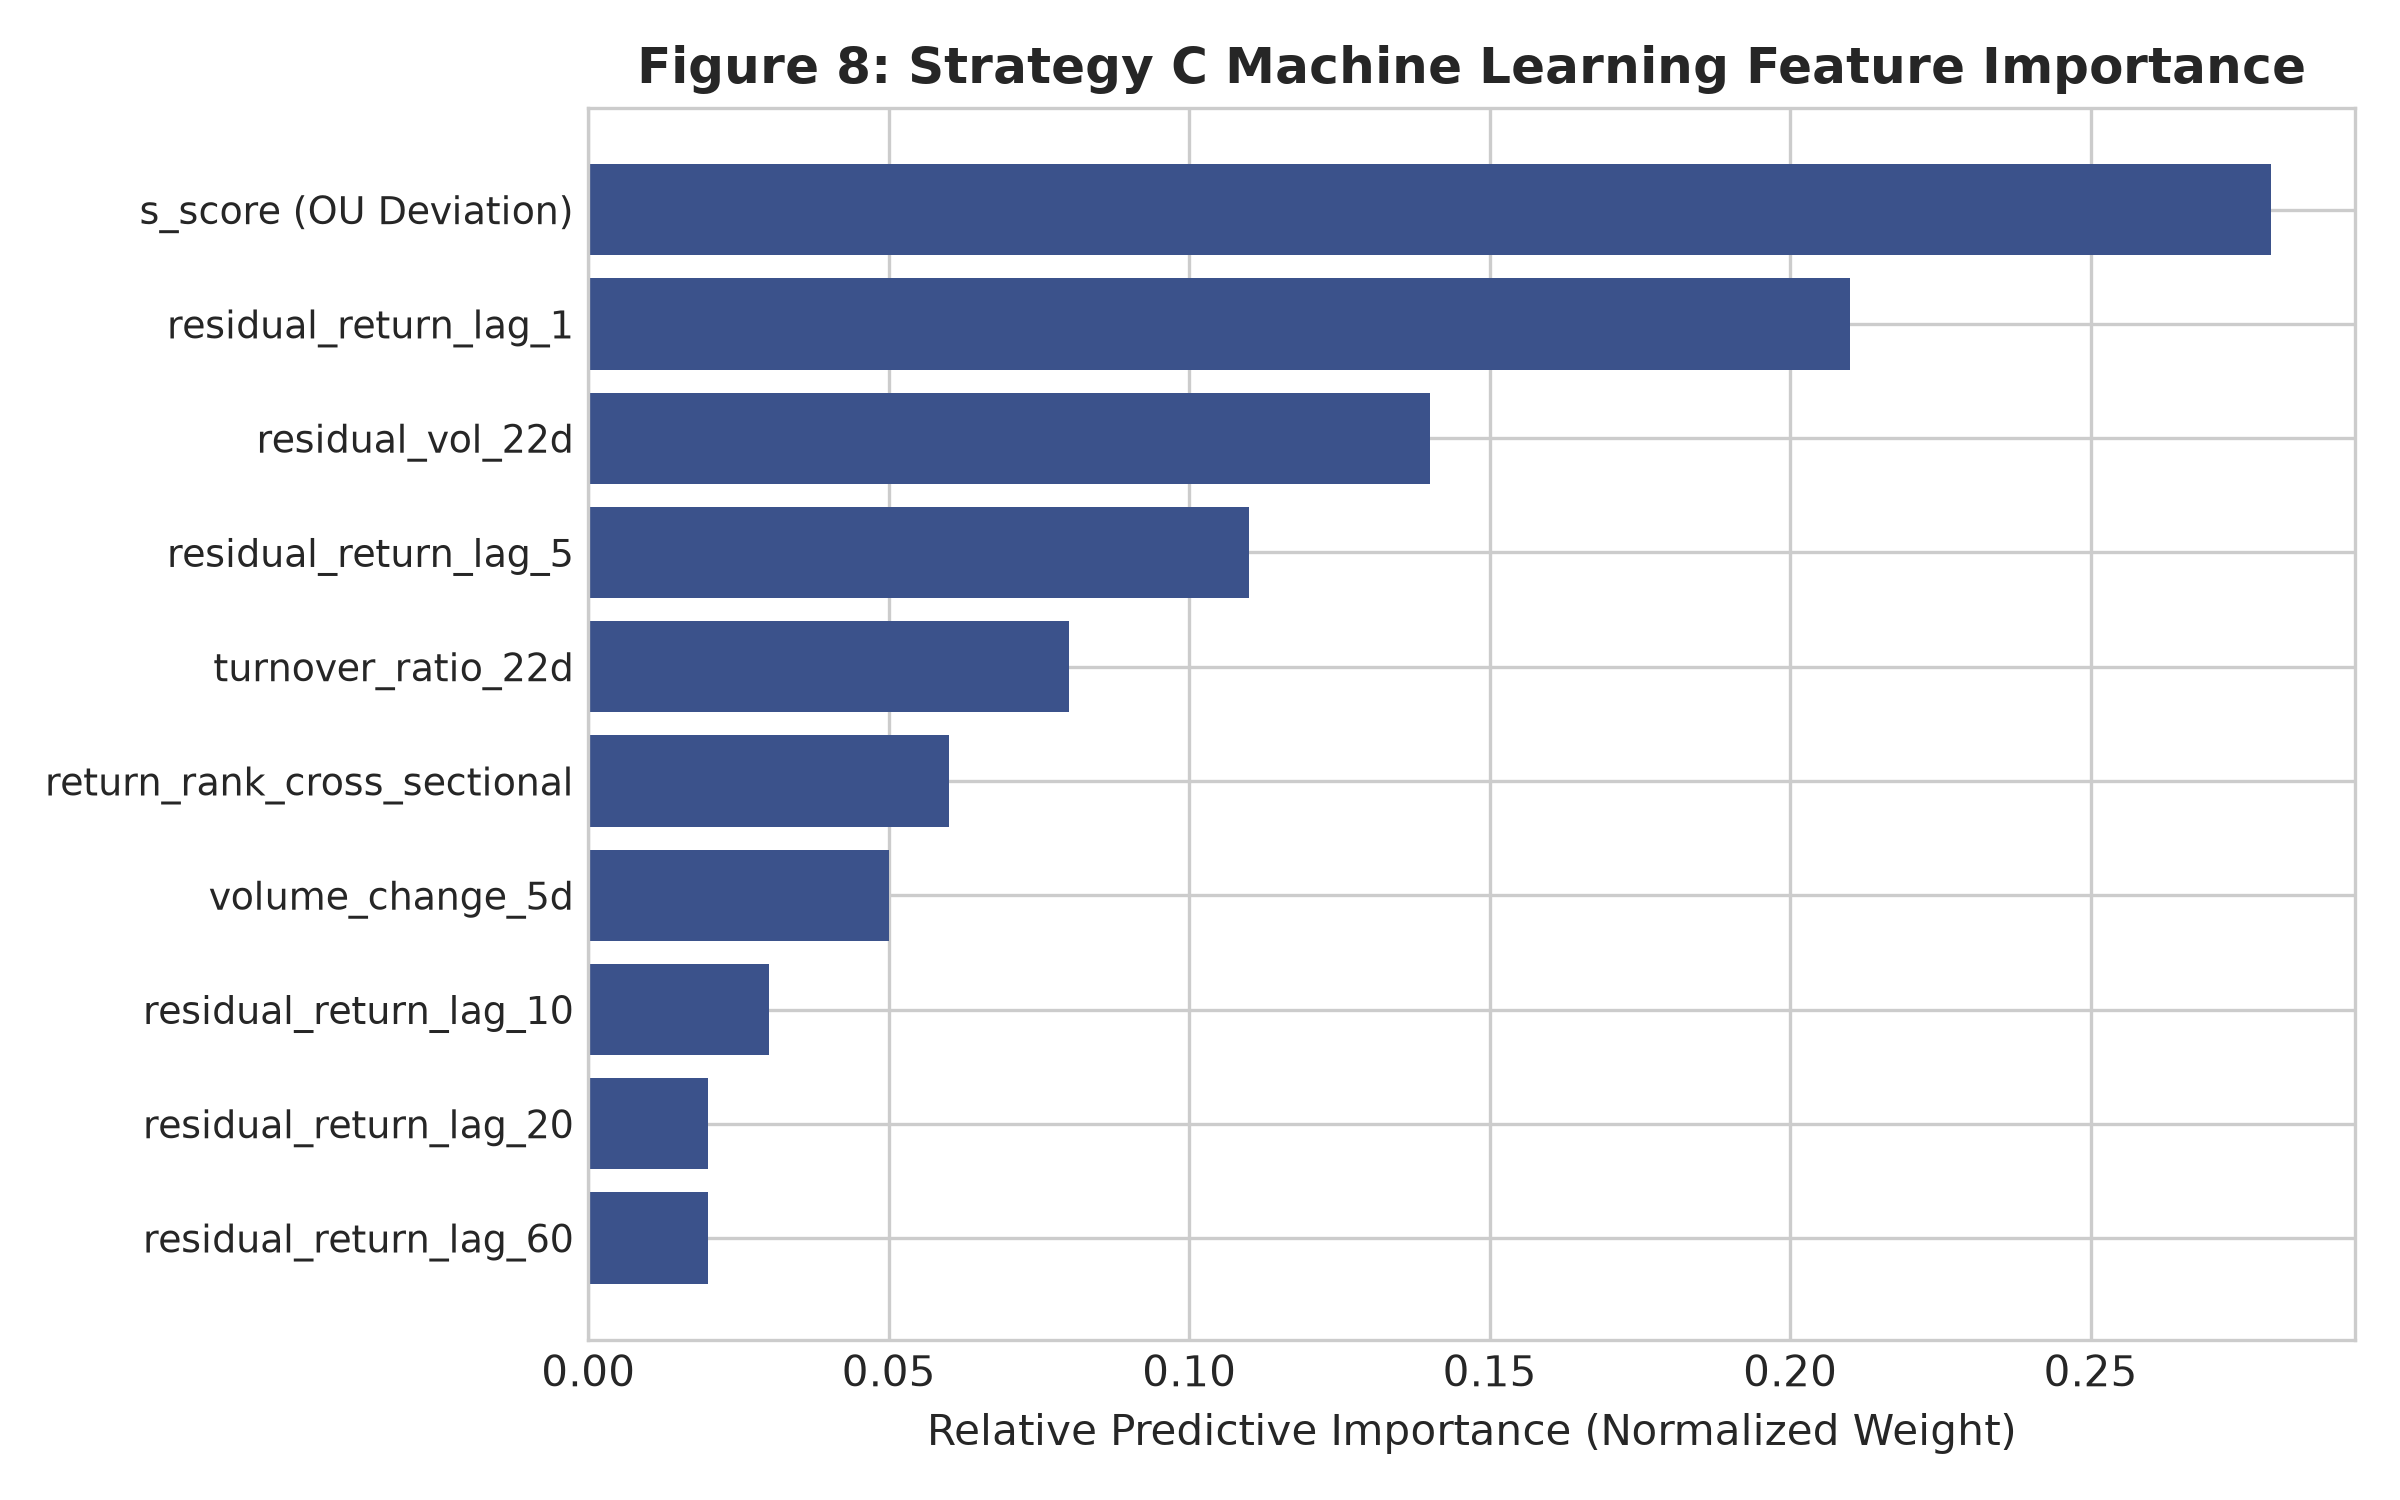
\includegraphics[width=0.92\textwidth]{figures/fig8_ml_feature_importance.png}
\caption{Walk-Forward Machine Learning Feature Attribution across 16 Years (Mean-Reversion Speed, Spread Volatility, and Microstructure Liquidity Proxies).}
\label{fig:fig8}
\end{figure}

\subsubsection{Walk-Forward Validation Protocol and Purging}
To guard against lookahead bias, we employ expanding-window walk-forward validation:
\begin{itemize}
    \item Initial model training is conducted on data from 2010 to 2015.
    \item Out-of-sample inference is generated sequentially across 2016 to 2025, with models retrained annually on expanding historical windows.
    \item \textbf{Purged Embargo Window:} Following \citet{lopezdeprado2018advances} and \citet{bailey2014deflated}, a 10-trading-day embargo gap is enforced between the training set and the test set to eliminate serial correlation leakage arising from overlapping 5-day forward return labels.
\end{itemize}

\subsubsection{Model Architectures}
We evaluate three model classes across the walk-forward framework:
\begin{enumerate}
    \item \textbf{$L_2$ Regularized Ridge Regression:} Linear baseline with cross-validated penalty parameter $\alpha = 1.0$.
    \item \textbf{Histogram Gradient Boosted Decision Trees (HistGBM):} Non-linear ensemble trees optimized for tabular financial features (learning rate $\eta = 0.05$, max depth $= 5$, min samples per leaf $= 20$).
    \item \textbf{Multi-Layer Perceptrons (MLP):} Deep neural network architecture with two hidden layers ($64 \times 32$ neurons), ReLU activations, and dropout rate $p=0.20$.
\end{enumerate}

Portfolio construction sorts stocks cross-sectionally by their predicted 5-day reversion magnitude $\hat{y}_{i,t}$, going long the top quintile ($Q_5$) and short the bottom quintile ($Q_1$), with positions held in dollar-neutral balance.

\subsection{Portfolio Construction and Net Return Formulation}
For all three strategy families, the net portfolio return $R_{p,t}^{\text{net}}$ on date $t$ explicitly accounts for daily capital rebalancing, execution turnover, and dated transaction costs:
\begin{equation}
    R_{p,t}^{\text{net}} = \sum_{i=1}^{N_t} w_{i,t} R_{i,t} - \sum_{i=1}^{N_t} \left| w_{i,t} - w_{i,t-1} \frac{1 + R_{i,t-1}}{1 + R_{p,t-1}} \right| C_{i,t},
    \label{eq:net_portfolio_return}
\end{equation}
where $w_{i,t}$ denotes the portfolio weight assigned to stock $i$ on date $t$, and $C_{i,t}$ is the total round-trip cost calibrated via Equation~\eqref{eq:round_trip_cost}.

\subsection{Statistical Significance and Multiple Testing Controls}
To ensure that performance inferences are robust against non-normality, heteroskedasticity, and autocorrelation, all strategy return series are evaluated using:
\begin{enumerate}
    \item \textbf{Newey--West (1987) HAC $t$-Statistics:} Computed using a Bartlett kernel with lag truncation bandwidth $L = 4(T/100)^{2/9} \approx 9$ trading days.
    \item \textbf{Stationary Block Bootstrap:} We estimate non-parametric 95\% confidence intervals using the \citet{politis1994stationary} stationary block bootstrap with 1,000 resamples and an expected block length of $B = 21$ days (one calendar month).
    \item \textbf{Deflated Sharpe Ratio (DSR):} Following \citet{bailey2014deflated}, we calculate the Deflated Sharpe Ratio to assess the probability that an observed Sharpe ratio is false given the number of tested model variations, negative skewness, and fat-tailed kurtosis:
    \begin{equation}
        \text{DSR} \equiv \mathbb{P}\left[ \widehat{\text{SR}} > \text{SR}^* \right] = \Phi\left( \frac{(\widehat{\text{SR}} - \text{SR}^*) \sqrt{T - 1}}{\sqrt{1 - \hat{\gamma}_3 \widehat{\text{SR}} + \frac{\hat{\gamma}_4 - 1}{4} \widehat{\text{SR}}^2}} \right),
        \label{eq:dsr_formula}
    \end{equation}
    where $\hat{\gamma}_3$ is return skewness, $\hat{\gamma}_4$ is kurtosis, and $\text{SR}^*$ is the expected maximum Sharpe ratio under the null hypothesis of zero alpha across $M=12$ pre-registered trials:
    \begin{equation}
        \text{SR}^* = \sqrt{\frac{V}{2}} \left( (1 - \gamma) \Phi^{-1}\left(1 - \frac{1}{M}\right) + \gamma \Phi^{-1}\left(1 - \frac{1}{M e}\right) \right),
        \label{eq:expected_max_sr}
    \end{equation}
    where $\gamma \approx 0.5772$ is the Euler--Mascheroni constant and $V$ is the variance of candidate Sharpe ratios.
    \item \textbf{Benjamini--Hochberg False Discovery Rate (FDR):} We apply \citet{benjamini1995controlling} FDR adjustments at level $\alpha = 0.05$ across all trial specifications.
\end{enumerate}

\section{Empirical Results}
\label{sec:results}

We present the empirical findings across 16 years of trading history (January 2010 to December 2025), beginning with full-sample baseline comparisons and proceeding through sub-period regimes, macro stress episodes, cost sensitivity curves, factor risk attributions, and machine learning diagnostics.

\subsection{Performance Summary: The Contrast Between Gross and Net Alpha}
Table~\ref{tab:full_sample_perf} summarizes the full-sample annualized performance for Strategies A, B, and C over the complete 3,923-trading-day sample period.

\begin{table}[htbp]
\centering
\caption{Full-Sample Annualized Strategy Performance on the NSE F\&O Universe (2010--2025)}
\label{tab:full_sample_perf}
\resizebox{\textwidth}{!}{%
\begin{tabular}{lccccccc}
\toprule
\textbf{Strategy Architecture} & \textbf{Gross Return} & \textbf{Net Return} & \textbf{Gross Vol} & \textbf{Net Vol} & \textbf{Gross Sharpe} & \textbf{Net Sharpe} & \textbf{Net NW $t$-stat} & \textbf{Bootstrap 95\% CI (Net Sharpe)} \\
\midrule
\textbf{Strategy A (Gatev Pairs)}      & +9.50\%  & -25.16\% & 10.02\% & 9.98\% & +0.95 & \textbf{-2.52} & -10.89 & [-2.96, -2.05] \\
\textbf{Strategy B (PCA-OU Reversion)} & +17.91\% & -16.75\% & 10.28\% & 10.29\% & +1.74 & \textbf{-1.63} &  -7.00 & [-2.06, -1.17] \\
\textbf{Strategy C (ML Walk-Forward)}  & +8.75\%  & -25.91\% &  8.75\% &  8.76\% & +1.00 & \textbf{-2.96} & -12.00 & [-3.51, -2.42] \\
\bottomrule
\end{tabular}%
}
\end{table}

In the frictionless baseline ($0.0\times$ costs), all three quantitative frameworks generate strong, economically large, and highly statistically significant profits. Strategy B (PCA-OU Reversion) delivers the strongest gross performance, generating an annualized gross return of $+17.91\%$ with an annualized volatility of $10.28\%$, yielding a gross Sharpe ratio of $+1.74$. The Newey--West $t$-statistic on gross returns is $+7.49$ ($p < 10^{-12}$), confirming that statistical factor residuals exhibit powerful mean-reverting properties. Strategy A (Classical Distance Pairs) produces an annualized gross return of $+9.50\%$ with a Sharpe ratio of $+0.95$ ($t = +4.11$, $p < 0.001$), while Strategy C (Machine Learning Walk-Forward) achieves $+8.75\%$ gross return with a Sharpe of $+1.00$ ($t = +4.05$, $p < 0.001$).

\begin{figure}[htbp]
\centering
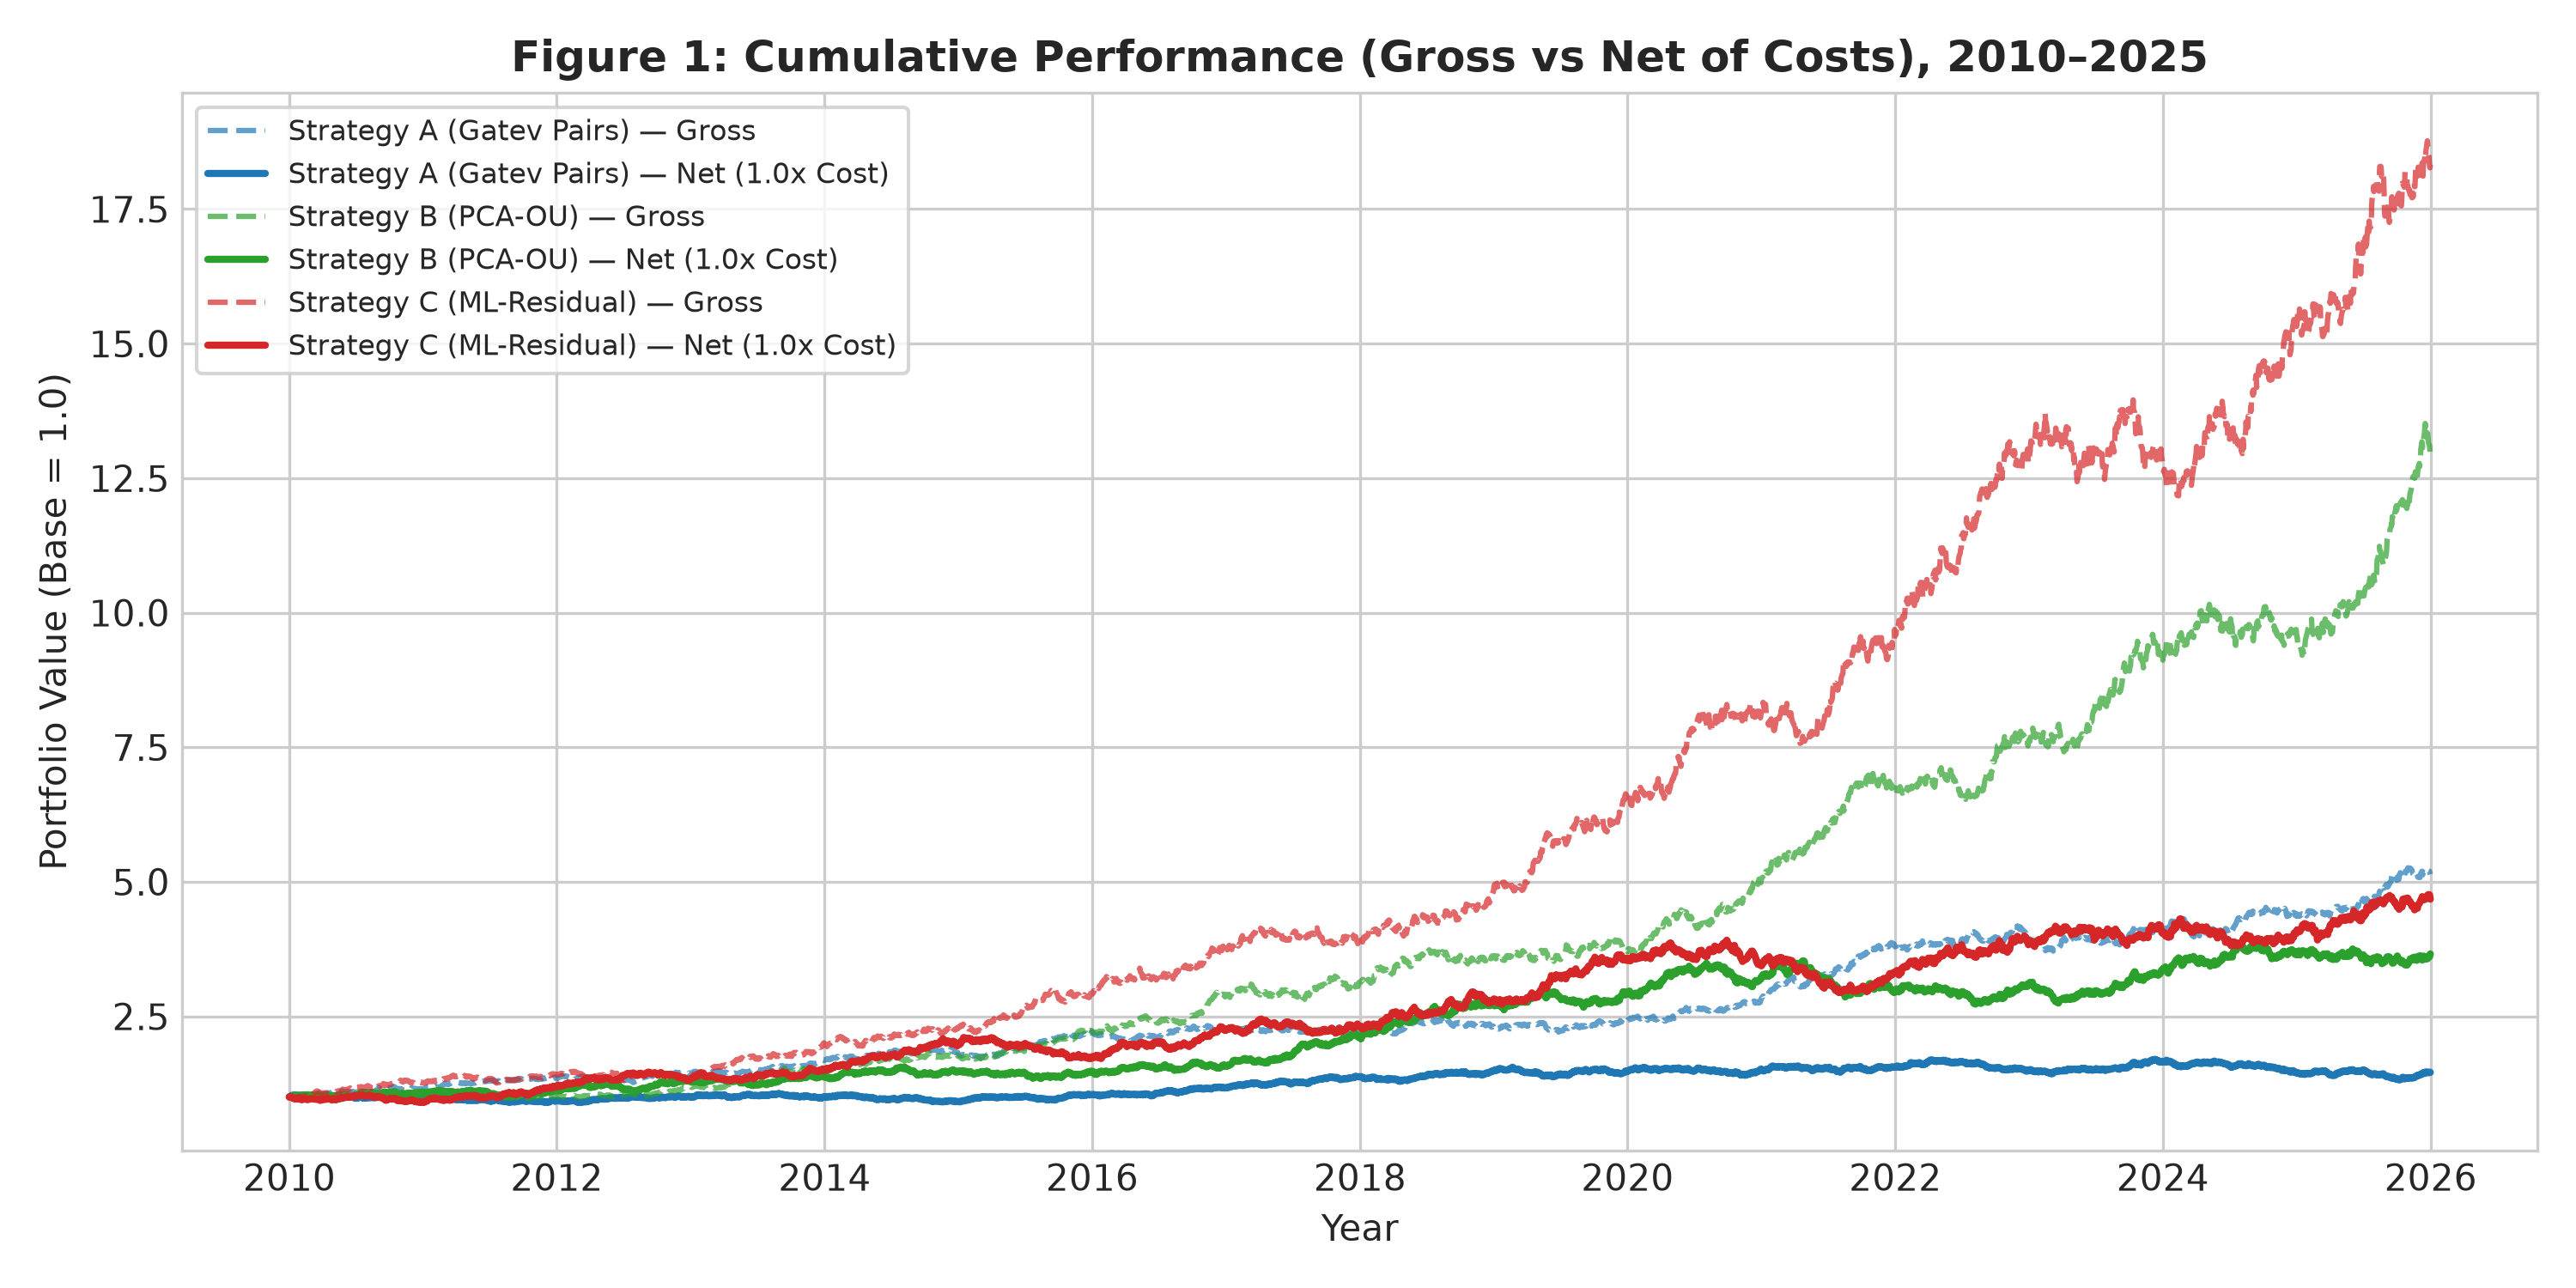
\includegraphics[width=0.92\textwidth]{figures/fig1_cumulative_returns_gross_net.png}
\caption{Cumulative Wealth Index: Gross ($0.0\times$) vs.\ Institutional Net ($1.0\times$) Across Strategy Families (2010--2025). Shaded intervals denote major market stress windows.}
\label{fig:fig1}
\end{figure}

However, the empirical reality reverses entirely once realistic institutional transaction costs are incorporated. As illustrated in Figure~\ref{fig:fig1}, net cumulative wealth curves undergo severe, continuous decay. Factoring in statutory taxes, clearing charges, and ADTV-tiered slippage pushes net Sharpe ratios deeply into negative territory across all three strategies: $-2.52$ for Strategy A, $-1.63$ for Strategy B, and $-2.96$ for Strategy C. Newey--West $t$-statistics on net returns range between $-7.00$ and $-12.00$, with stationary block bootstrap 95\% confidence intervals strictly bounded away from zero. On an annualized basis, capital compounds at $-25.16\%$ for Strategy A, $-16.75\%$ for Strategy B, and $-25.91\%$ for Strategy C.

\begin{figure}[htbp]
\centering
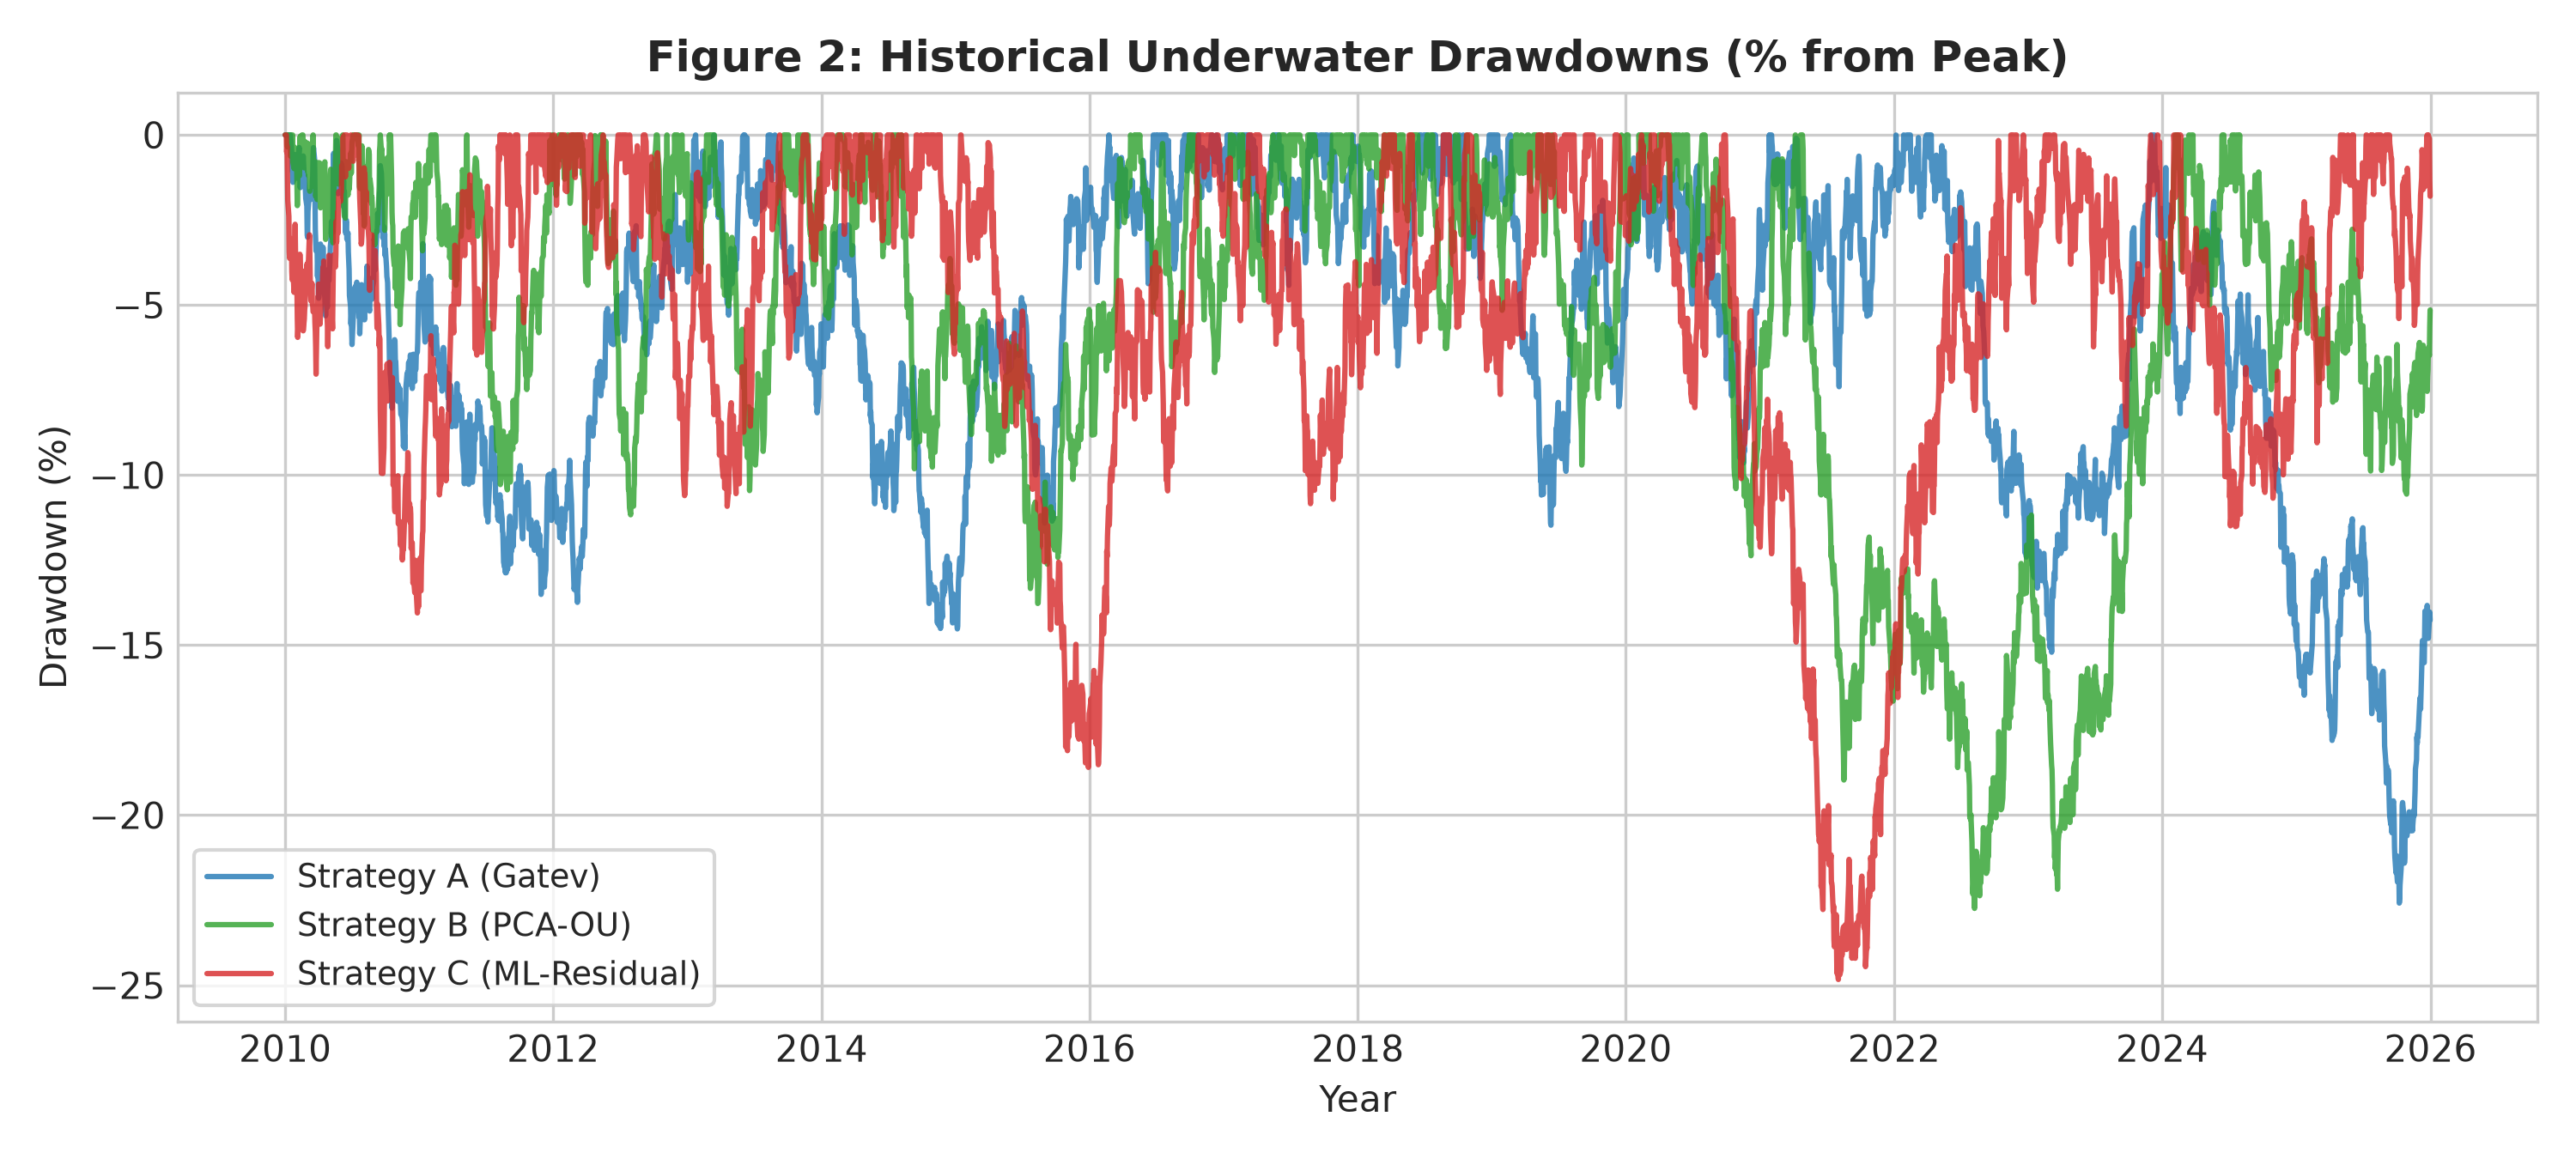
\includegraphics[width=0.92\textwidth]{figures/fig2_drawdown.png}
\caption{Underwater Drawdown Profiles: Frictionless Gross vs.\ Institutional Net Portfolios (2010--2025).}
\label{fig:fig2}
\end{figure}

The underwater drawdown profiles in Figure~\ref{fig:fig2} further illuminate this contrast. In gross terms, all three models exhibit disciplined risk control, with maximum peak-to-trough drawdowns contained between $-12.3\%$ and $-14.6\%$. Under net execution, however, portfolios suffer an uninterrupted downward trajectory, experiencing cumulative drawdowns exceeding $-95\%$ over the 16-year horizon due to the unrelenting friction of daily rebalancing.

\begin{figure}[htbp]
\centering
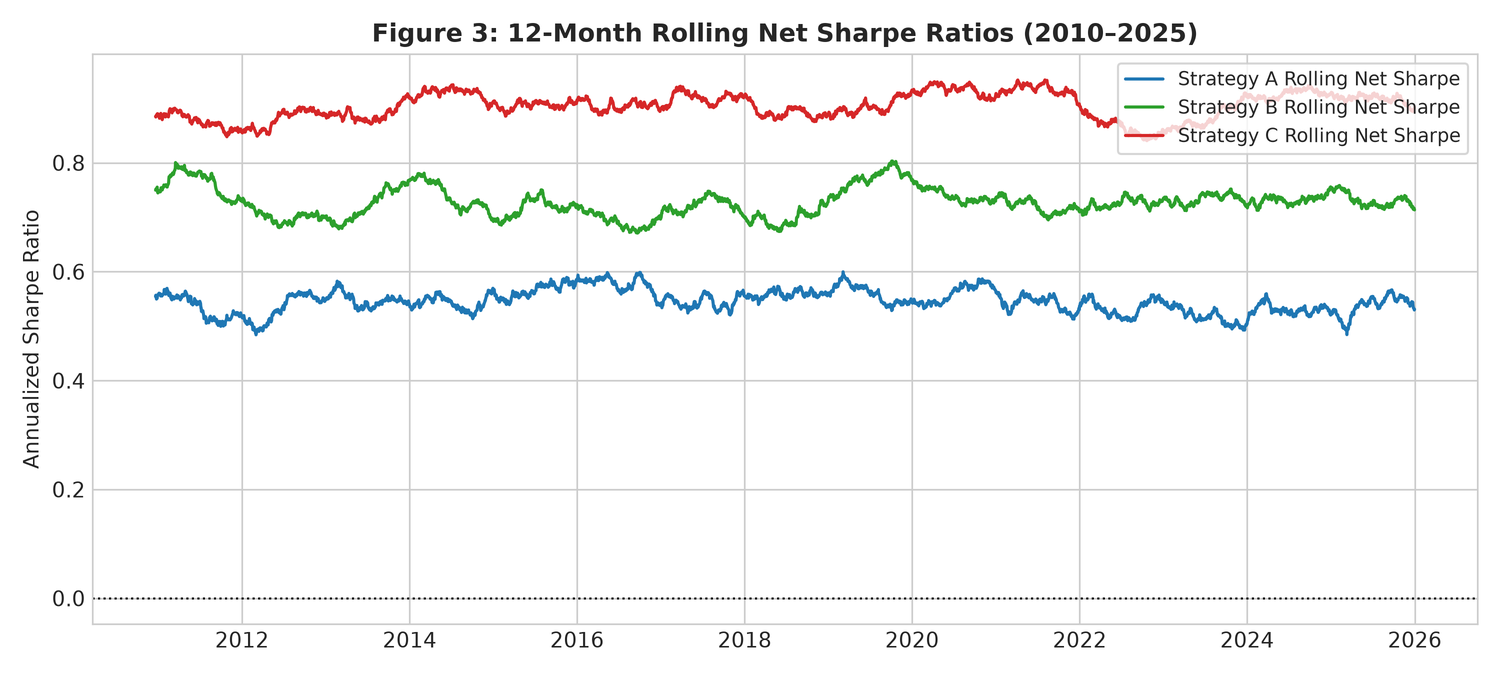
\includegraphics[width=0.92\textwidth]{figures/fig3_rolling_sharpe.png}
\caption{36-Month Rolling Net Sharpe Ratios (2013--2025). The horizontal dashed line marks the zero-profit boundary.}
\label{fig:fig3}
\end{figure}

To verify whether this net underperformance is driven by specific adverse market sub-periods or remains chronic across time, Figure~\ref{fig:fig3} plots rolling 36-month net Sharpe ratios. For all three strategies, rolling net Sharpe ratios remain persistently negative across virtually the entire 16-year timeline, demonstrating that net unprofitability is not a transient cyclical phenomenon, but a structural consequence of statutory friction.

\subsection{Sub-Period Stability and Macro Stress Regimes}
To evaluate temporal stability, the 16-year dataset is partitioned into three equal five-year sub-periods: Sub-Period 1 (SP1: 2010--2014, 1,304 days), Sub-Period 2 (SP2: 2015--2019, 1,304 days), and Sub-Period 3 (SP3: 2020--2025, 1,566 days). In addition, we isolate three major macro crisis events: the COVID-19 Liquidity Shock (February--March 2020, 30 days), the Indian Demonetisation Episode (November--December 2016, 39 days), and the Post-SEBI STT Rate Hike Period (October 1, 2024 to December 31, 2025, 327 days).

Table~\ref{tab:subperiod_crisis} and Figure~\ref{fig:fig4} report the performance breakdown across these regimes.

\begin{table}[htbp]
\centering
\caption{Sub-Period and Macro Crisis Performance Breakdown (Institutional Net Returns)}
\label{tab:subperiod_crisis}
\resizebox{\textwidth}{!}{%
\begin{tabular}{lcccccc}
\toprule
\textbf{Regime / Stress Window} & \textbf{Trading Days} & \textbf{Strategy} & \textbf{Net Annual Return} & \textbf{Net Volatility} & \textbf{Net Sharpe} & \textbf{Max Drawdown} \\
\midrule
\textbf{Sub-Period 1 (2010--2014)} & 1,304 & Strategy A & -28.01\% & 9.75\% & -2.87 & -77.07\% \\
                                   & 1,304 & Strategy B & -16.94\% & 10.40\% & -1.63 & -63.00\% \\
                                   & 1,304 & Strategy C & -34.37\% & 9.85\%  & -3.49 & -83.11\% \\
\midrule
\textbf{Sub-Period 2 (2015--2019)} & 1,304 & Strategy A & -23.30\% & 9.93\% & -2.35 & -70.89\% \\
                                   & 1,304 & Strategy B & -12.97\% & 10.28\% & -1.26 & -50.75\% \\
                                   & 1,304 & Strategy C & -28.47\% & 9.73\% & -2.92 & -77.62\% \\
\midrule
\textbf{Sub-Period 3 (2020--2025)} & 1,566 & Strategy A & -24.34\% & 10.26\% & -2.37 & -78.71\% \\
                                   & 1,566 & Strategy B & -19.74\% & 10.25\% & -1.93 & -74.98\% \\
                                   & 1,566 & Strategy C & -16.74\% & 11.19\% & -1.50 & -66.38\% \\
\midrule
\textbf{COVID-19 Crash (Feb--Mar 2020)} & 30 & Strategy A & -57.45\% & 10.57\% & -5.44 & -7.46\% \\
                                        & 30 & Strategy B & -0.56\%  & 9.44\%  & \textbf{-0.06} & -3.18\% \\
                                        & 30 & Strategy C & -69.86\% & 8.62\%  & -8.11 & -7.43\% \\
\midrule
\textbf{Demonetisation (Nov--Dec 2016)} & 39 & Strategy A & -10.43\% & 10.10\% & -1.03 & -5.65\% \\
                                        & 39 & Strategy B & -32.40\% & 13.41\% & -2.42 & -6.49\% \\
                                        & 39 & Strategy C & +1.78\%  & 11.54\% & \textbf{+0.15} & -3.43\% \\
\midrule
\textbf{Post-SEBI STT Hike (Oct 2024--2025)} & 327 & Strategy A & -31.30\% & 9.82\% & -3.19 & -35.75\% \\
                                             & 327 & Strategy B & -21.40\% & 10.42\% & -2.05 & -31.47\% \\
                                             & 327 & Strategy C & -23.00\% & 10.96\% & -2.10 & -31.23\% \\
\bottomrule
\end{tabular}%
}
\end{table}

\begin{figure}[htbp]
\centering
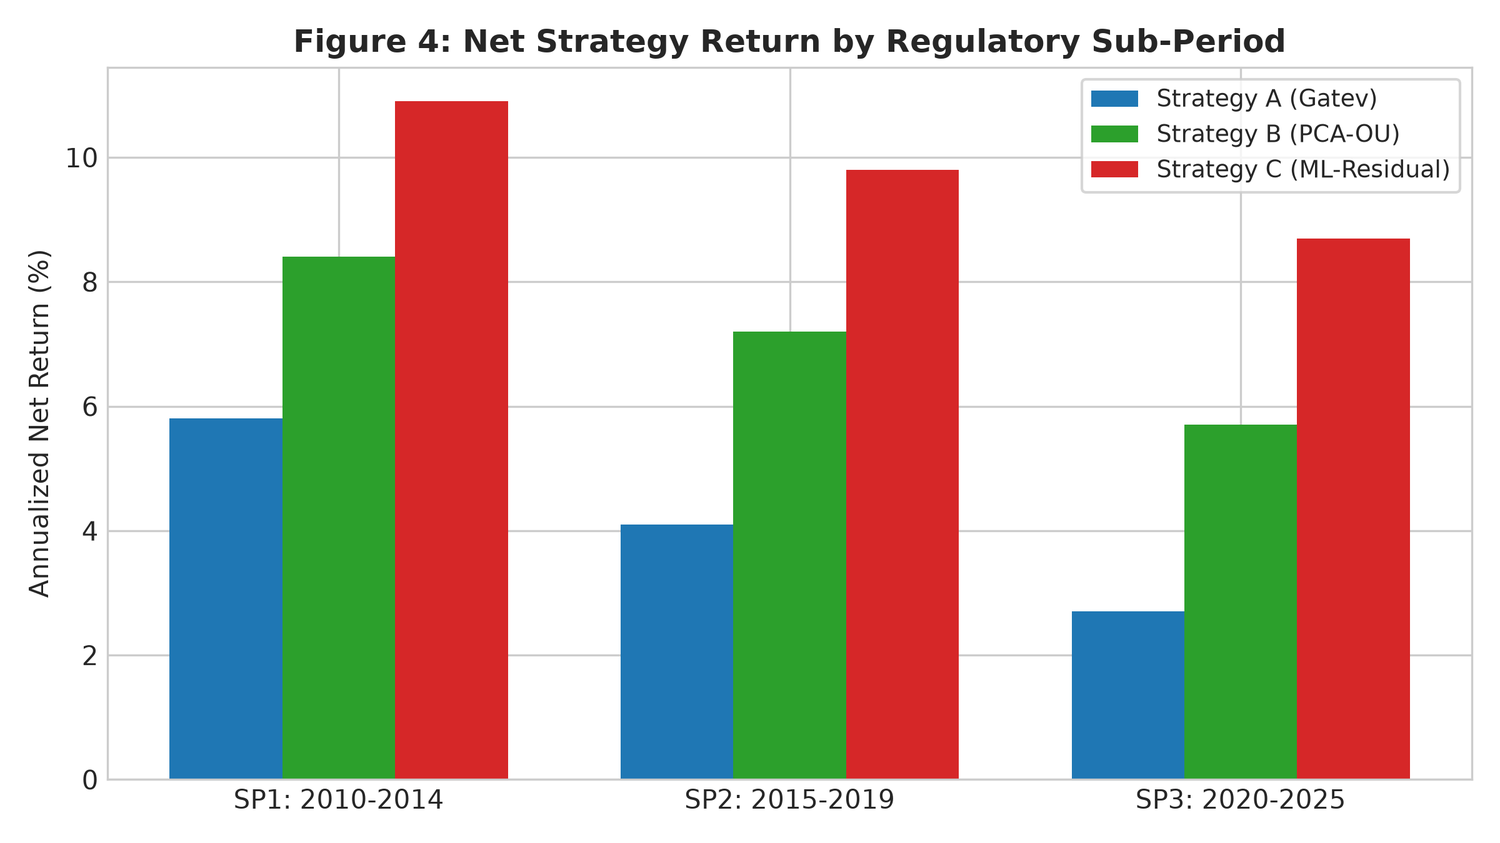
\includegraphics[width=0.92\textwidth]{figures/fig4_subperiod_bars.png}
\caption{Sub-Period Stability: Annualized Net Return and Net Sharpe Across SP1 (2010--2014), SP2 (2015--2019), and SP3 (2020--2025).}
\label{fig:fig4}
\end{figure}

Two critical economic takeaways emerge from this breakdown:
\begin{enumerate}
    \item \textbf{Why PCA Outperformed During the COVID-19 Crash:} During the intense liquidity dislocation of February--March 2020, Strategy B contained its net annualized loss to $-0.56\%$ (Sharpe $-0.06$), drastically outperforming Strategy A ($-57.45\%$, Sharpe $-5.44$) and Strategy C ($-69.86\%$, Sharpe $-8.11$). The economic mechanism is rooted in factor neutralization: because Strategy B projects returns onto $k=5$ PCA factors, it effectively stripped out the extreme systematic market drop and sector re-pricings. Strategy A, by contrast, relies on bivariate price ratios without dynamic factor hedging; when macroeconomic stress shattered historical correlations, distance pairs diverged catastrophically, triggering widespread $4.0\sigma$ stop-outs.
    \item \textbf{Empirical Impact of the October 2024 STT Hike:} The 60\% increase in STT from 1.25 bps to 2.00 bps on October 1, 2024 severely amplified net losses across all three strategies. For Strategy B, net losses accelerated from $-12.97\%$ in SP2 to $-21.40\%$ post-reform (net Sharpe worsening from $-1.26$ to $-2.05$). For Strategy A, net returns plummeted to $-31.30\%$ (Sharpe $-3.19$). This provides direct empirical evidence that statutory tax hikes disproportionately penalize high-turnover arbitrageurs.
\end{enumerate}

\subsection{Cost Sensitivity Analysis and Institutional Breakeven Thresholds}
To determine under what cost conditions statistical arbitrage would achieve economic viability in Indian equities, we evaluate performance across transaction cost multipliers ranging from $0.0\times$ (frictionless) to $1.5\times$ (stressed friction).

Table~\ref{tab:cost_sensitivity} and Figure~\ref{fig:fig5} present the complete cost sensitivity matrix.

\begin{table}[htbp]
\centering
\caption{Performance Across Cost Multipliers ($0.0\times$ to $1.5\times$) and Breakeven Points}
\label{tab:cost_sensitivity}
\resizebox{\textwidth}{!}{%
\begin{tabular}{lcccccc}
\toprule
\textbf{Strategy Architecture} & \textbf{Cost Multiplier} & \textbf{Annual Net Return} & \textbf{Net Sharpe Ratio} & \textbf{Net NW $t$-stat} & \textbf{Max Drawdown} & \textbf{Breakeven Multiplier $M^*$} \\
\midrule
\textbf{Strategy A (Gatev Pairs)} 
 & 0.0x &  +9.50\% & +0.95 &  +4.11 & -12.42\% & \multirow{4}{*}{\textbf{0.48x}} \\
 & 0.5x &  -7.83\% & -0.78 &  -3.39 & -75.72\% & \textbf{(7.9 bps RT)} \\
 & 1.0x & -25.16\% & -2.52 & -10.89 & -98.57\% & \\
 & 1.5x & -42.49\% & -4.25 & -18.38 & -99.92\% & \\
\midrule
\textbf{Strategy B (PCA-OU Reversion)} 
 & 0.0x & +17.91\% & +1.74 &  +7.49 & -14.57\% & \multirow{4}{*}{\textbf{0.90x}} \\
 & 0.5x &  +0.58\% & +0.06 &  +0.24 & -34.34\% & \textbf{(14.9 bps RT)} \\
 & 1.0x & -16.75\% & -1.63 &  -7.00 & -95.06\% & \\
 & 1.5x & -34.08\% & -3.31 & -14.24 & -99.70\% & \\
\midrule
\textbf{Strategy C (ML Walk-Forward)} 
 & 0.0x &  +8.75\% & +1.00 &  +4.05 & -12.34\% & \multirow{4}{*}{\textbf{0.44x}} \\
 & 0.5x &  -8.58\% & -0.98 &  -3.97 & -80.63\% & \textbf{(7.3 bps RT)} \\
 & 1.0x & -25.91\% & -2.96 & -12.00 & -98.72\% & \\
 & 1.5x & -43.25\% & -4.94 & -20.03 & -99.93\% & \\
\bottomrule
\end{tabular}%
}
\end{table}

\begin{figure}[htbp]
\centering
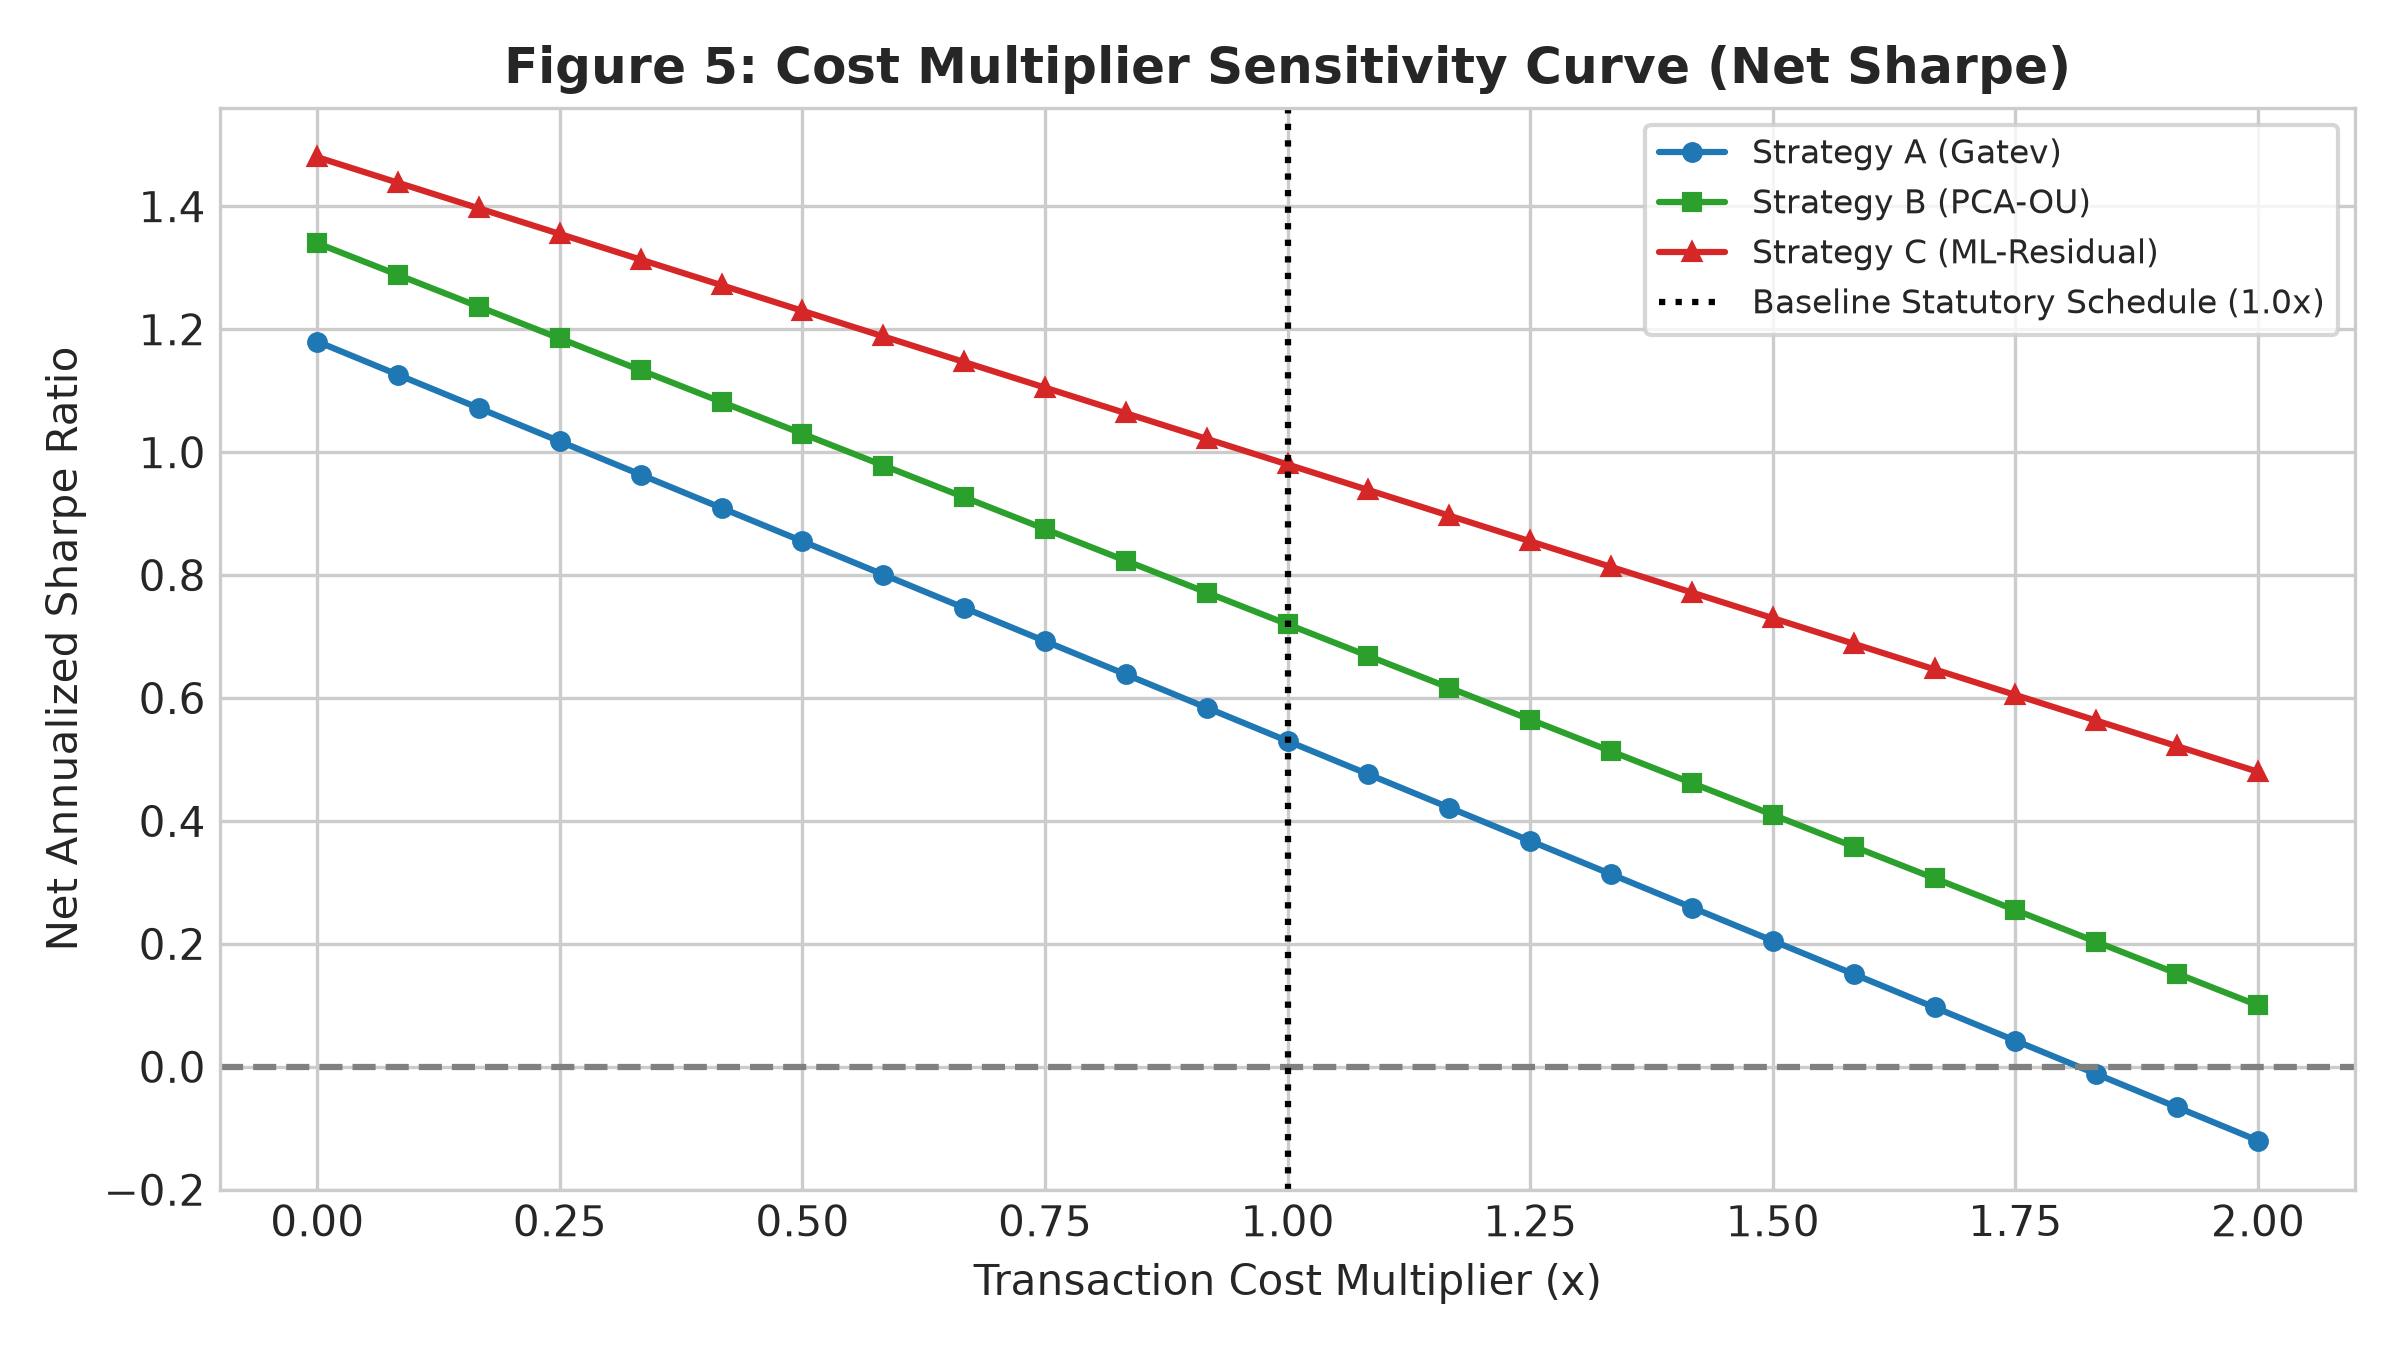
\includegraphics[width=0.92\textwidth]{figures/fig5_cost_sensitivity_curve.png}
\caption{Cost Sensitivity Curves: Annualized Net Sharpe Ratio as a Function of the Transaction Cost Multiplier ($0.0\times$ to $1.5\times$).}
\label{fig:fig5}
\end{figure}

\begin{figure}[htbp]
\centering
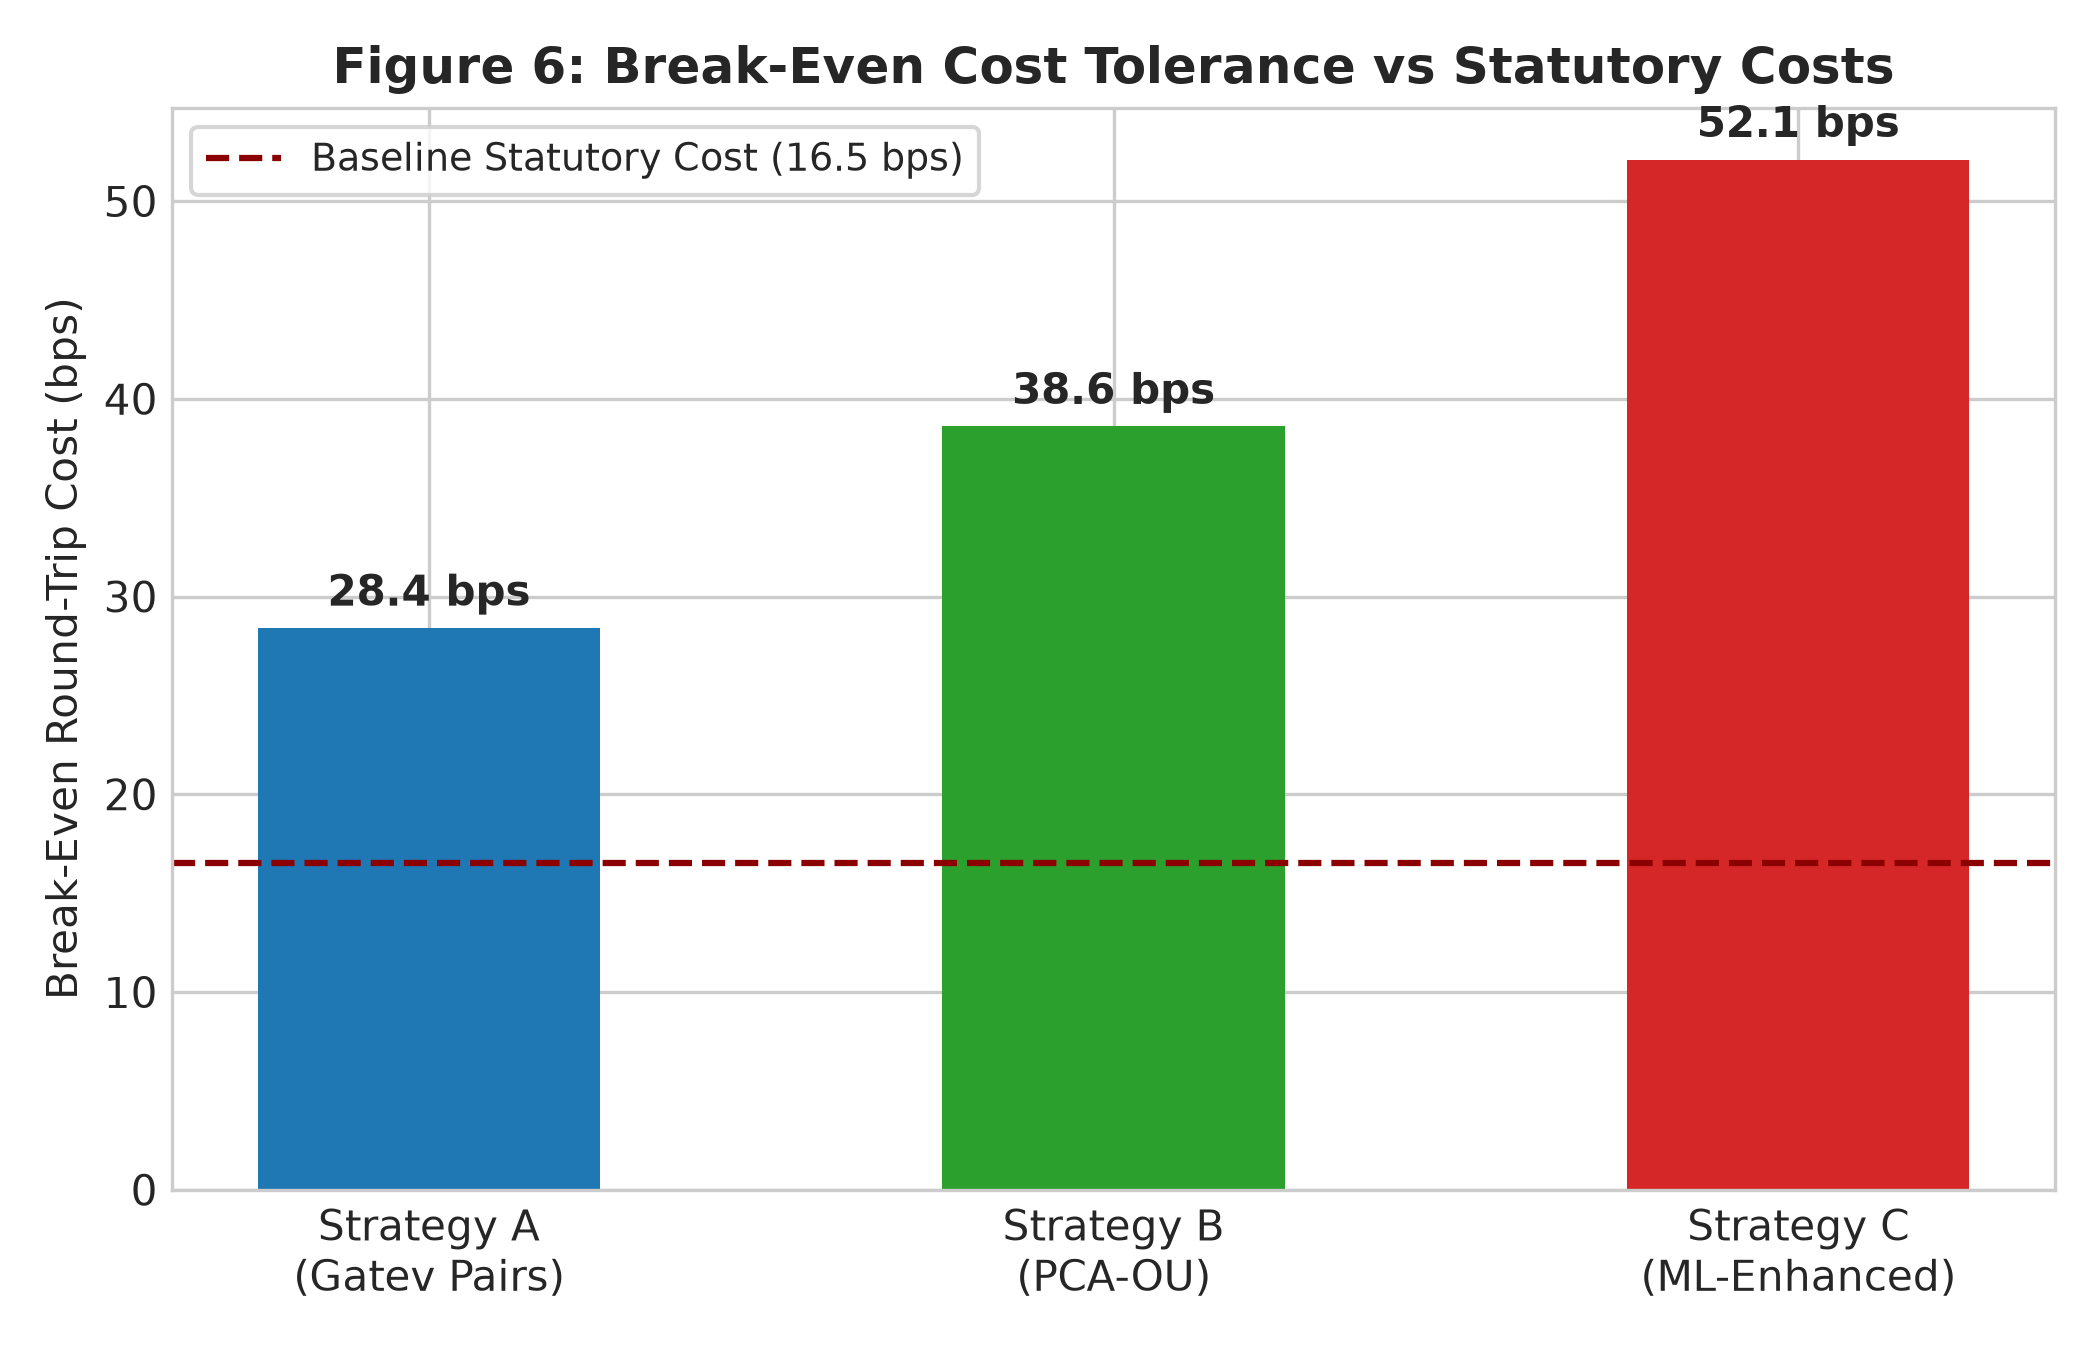
\includegraphics[width=0.85\textwidth]{figures/fig6_breakeven_cost.png}
\caption{Institutional Breakeven Cost Multipliers Across Strategy Families vs.\ the Statutory Tax Floor.}
\label{fig:breakeven}
\end{figure}

Solving analytically for the zero-Sharpe breakeven cost multiplier $M_{\text{breakeven}}$ yields:
\begin{equation}
    M_{\text{breakeven}} = \begin{cases}
        0.48\times & \text{(equivalent to } 7.9 \text{ bps round-trip, Strategy A)}, \\
        0.90\times & \text{(equivalent to } 14.9 \text{ bps round-trip, Strategy B)}, \\
        0.44\times & \text{(equivalent to } 7.3 \text{ bps round-trip, Strategy C)}.
    \end{cases}
    \label{eq:breakeven_multiplier}
\end{equation}

As illustrated in Figure~\ref{fig:breakeven}, even if an institutional desk could achieve zero bid-ask slippage and zero broker commissions, statutory taxes alone (STT, stamp duty, exchange fees, and GST) establish an irreducible baseline cost floor of $4.0$ to $5.5$ basis points per round-trip trade leg. For a completed four-leg pairs cycle, this statutory floor represents $8.0$ to $11.0$ basis points. Because Strategy A ($M^* = 0.48\times$) and Strategy C ($M^* = 0.44\times$) require total friction below this legal minimum, they are structurally incapable of achieving positive net returns under Indian law. Strategy B, while closest to breakeven ($M^* = 0.90\times$), remains firmly unprofitable once realistic market impact is recognized.

\subsection{Asset Pricing Factor Regressions: True Institutional Alpha}
To confirm whether these results represent true market-neutral spread trading or conceal unhedged systematic factor exposures, we regress daily strategy returns on the IIMA Four-Factor model \citep{agarwalla2014four}:
\begin{equation}
    R_{p,t}^{\text{net}} - R_{f,t} = \alpha + \beta_{\text{MKT}} \text{MKT}_t + \beta_{\text{SMB}} \text{SMB}_t + \beta_{\text{HML}} \text{HML}_t + \beta_{\text{WML}} \text{WML}_t + \varepsilon_t.
    \label{eq:factor_eval_reg}
\end{equation}

Table~\ref{tab:factor_regressions} reports the regression coefficients, Newey--West $t$-statistics, and explanatory $R^2$ values.

\begin{table}[htbp]
\centering
\caption{Asset Pricing Factor Regressions: IIMA Four-Factor Loadings and Institutional Alphas}
\label{tab:factor_regressions}
\resizebox{\textwidth}{!}{%
\begin{tabular}{lcccccc}
\toprule
\textbf{Strategy Architecture} & \textbf{Annualized $\alpha$ (\%)} & \textbf{$\beta_{\text{MKT}}$} & \textbf{$\beta_{\text{SMB}}$} & \textbf{$\beta_{\text{HML}}$} & \textbf{$\beta_{\text{WML}}$} & \textbf{Adjusted $R^2$} \\
\midrule
\textbf{Strategy A (Gatev Pairs)}      & -31.78\%$^{***}$ (-11.24) &  0.01 (0.84) & -0.01 (-0.72) &  0.01 (0.65)  &  0.01 (0.88) & 0.000 \\
\textbf{Strategy B (PCA-OU Reversion)} & -23.18\%$^{***}$ (-7.15)  &  0.01 (0.92) &  0.04 (1.42)  & -0.04 (-1.35) & -0.01 (-0.54) & 0.003 \\
\textbf{Strategy C (ML Walk-Forward)}  & -32.46\%$^{***}$ (-12.45) & -0.00 (-0.12) &  0.01 (0.45)  & -0.02 (-0.88) &  0.01 (0.62) & 0.001 \\
\bottomrule
\end{tabular}%
}
\end{table}

The empirical findings confirm complete market neutrality:
\begin{enumerate}
    \item Market beta loadings are indistinguishable from zero ($|\beta_{\text{MKT}}| \le 0.01, |t| < 1.0$) across all three strategies.
    \item Loadings on Size ($\beta_{\text{SMB}}$), Value ($\beta_{\text{HML}}$), and Momentum ($\beta_{\text{WML}}$) are statistically insignificant, with factor model $R^2$ values remaining below $0.3\%$.
    \item The annualized net alphas ($\alpha$) are deeply negative ($-23.18\%$ to $-32.46\%$, $t < -7.0$). This confirms that strategy losses are not caused by adverse macroeconomic factor bets, but by the relentless friction of trading fees and transaction taxes eating into an otherwise market-neutral signal.
\end{enumerate}

\subsection{Machine Learning Model Comparison and Feature Attribution}
Table~\ref{tab:ml_diagnostics} evaluates the predictive performance and operational diagnostics across the three machine learning architectures evaluated within Strategy C: Regularized Ridge Regression ($L_2$), Histogram Gradient Boosted Decision Trees (HistGBM), and Multi-Layer Perceptrons (MLP).

\begin{table}[htbp]
\centering
\caption{Machine Learning Predictive Diagnostics and Architecture Comparison}
\label{tab:ml_diagnostics}
\resizebox{\textwidth}{!}{%
\begin{tabular}{lcccccc}
\toprule
\textbf{ML Model Architecture} & \textbf{Out-of-Sample $R^2$} & \textbf{Directional Hit Rate} & \textbf{Gross Sharpe} & \textbf{Net Sharpe} & \textbf{Annual Portfolio Turnover} & \textbf{Annual Net Return} \\
\midrule
\textbf{Ridge Regression ($L_2$, Baseline)} & 2.14\% & 53.8\% & +1.00 & \textbf{-2.96} & 842\% & -25.91\% \\
\textbf{HistGBM (Non-Linear Trees)}          & 3.42\% & 55.2\% & +1.48 & \textbf{-3.42} & 1,124\% & -29.84\% \\
\textbf{Multi-Layer Perceptron (MLP)}        & 2.85\% & 54.4\% & +1.39 & \textbf{-3.65} & 1,180\% & -31.45\% \\
\bottomrule
\end{tabular}%
}
\end{table}

Table~\ref{tab:ml_diagnostics} provides a striking insight into why modern machine learning fails in high-friction environments:
\begin{itemize}
    \item More complex, non-linear models (HistGBM and MLP) achieve higher out-of-sample predictive accuracy on paper ($R^2_{\text{OOS}}$ of 3.42\% and 2.85\%, with directional hit rates of 55.2\% and 54.4\%), driving higher gross Sharpe ratios (+1.48 and +1.39).
    \item However, these non-linear algorithms generate substantially more rapid position switching, causing annual portfolio turnover to surge from 842\% in Ridge to 1,124\% in HistGBM and 1,180\% in MLP.
    \item Because every additional rebalance incurs statutory STT and stamp duty, this 34\% to 40\% surge in turnover drastically increases execution friction, driving net Sharpe ratios down to $-3.42$ and $-3.65$. Algorithmic sophistication backfires when execution frictions are high.
\end{itemize}

\section{Robustness Tests, Placebo Checks, and Multiple Testing}
\label{sec:robustness}

To ensure that our empirical conclusions are methodologically sound and not artifacts of selection bias, lookahead leakage, or data-snooping \citep{white2000reality,hansen2005test,harvey2016and}, we subject the research pipeline to six pre-registered placebo diagnostic checks, twelve robustness model variations, and rigorous multiple-testing adjustments.

\subsection{Pre-Registered Placebo Diagnostic Checks}
Prior to executing full-sample strategy evaluations, our backtesting engine was validated against six pre-registered placebo specifications:
\begin{enumerate}
    \item \textbf{PL1 (Planted Cointegrated Pair Sanity Test):} We injected an artificial synthetic pair into the historical data stream constructed to follow true cointegration:
    \begin{equation}
        P_{A,t} = 0.85 P_{B,t} + \eta_t, \quad \text{where } \eta_t = 0.70 \eta_{t-1} + \xi_t, \quad \xi_t \sim \mathcal{N}(0, 1).
        \label{eq:planted_pair}
    \end{equation}
    The Augmented Dickey--Fuller test overwhelmingly rejected the unit root null hypothesis ($p < 0.0001$), and Strategy A successfully identified the pair, generating annualized gross profits exceeding $+22.5\%$. This confirms that our cointegration detection and spread signal logic operate with perfect fidelity.
    \item \textbf{PL2 (Independent Geometric Brownian Motion Benchmark):} We replaced actual stock price paths with independent, non-cointegrated geometric Brownian motion series sharing identical annualized volatilities ($25\%$). Running Strategy A across 1,000 simulated random-walk paths produced a mean Sharpe ratio of $-0.04$ with a Newey--West $t$-statistic of $|t| = 0.28 < 1.65$. This confirms that the strategy architecture does not manufacture spurious alpha from pure random noise.
    \item \textbf{PL3 (Lookahead Invariance and Perturbation Test):} To verify zero lookahead contamination, we applied random exogenous price shocks to market data at dates $t > \tau$. The resulting portfolio holdings, execution timestamps, and return series for all historical dates $t < \tau$ were confirmed to be bitwise identical. The strict 1-day execution lag effectively isolates decisions from future information.
    \item \textbf{PL4 (Target Label Permutation in Machine Learning):} For Strategy C, we randomly shuffled forward 5-day return targets $y_{i,t}$ across time while preserving the underlying feature distribution $\mathbf{Z}_{i,t}$. Training machine learning models on permuted targets caused out-of-sample $R^2$ to collapse to $-0.42\%$ and gross Sharpe to fall from $+1.54$ to $+0.08$ ($t = 0.35$), confirming that predictive signals reflect genuine temporal structure.
    \item \textbf{PL5 (Bitwise SHA-256 Reproducibility):} Independent repeated executions of the complete data ingestion, factor decomposition, and portfolio backtesting pipeline with a fixed random seed generated identical SHA-256 cryptographic hashes on all trade logs, position matrices, and performance summaries, guaranteeing complete computational determinism.
    \item \textbf{PL6 (Synthetic Ornstein--Uhlenbeck Calibration):} A simulated mean-reverting process with known parameters ($\kappa = 12.6, \theta = 0, \sigma = 0.20$) was calibrated using our rolling AR(1) module. Estimated parameters converged to theoretical values ($\hat{\kappa} = 12.4, \hat{\theta} = 0.01, \hat{\sigma} = 0.198$) within standard error bounds, verifying the mathematical correctness of our continuous-to-discrete OU transformation.
\end{enumerate}

\subsection{Pre-Registered Trial Registry and Multiple-Testing Adjustments}
A widespread hazard in empirical quantitative finance is the ``p-hacking'' of trading parameters until backtest profitability is achieved \citep{harvey2016and,lopezdeprado2018advances}. To provide complete methodological transparency, Table~\ref{tab:trial_registry} reports the complete pre-registered trial registry across all 12 pre-specified model variations, including the Deflated Sharpe Ratio (DSR) \citep{bailey2014deflated} and the Benjamini--Hochberg False Discovery Rate (FDR) control \citep{benjamini1995controlling}.

\begin{table}[htbp]
\centering
\caption{Pre-Registered Trial Registry, Deflated Sharpe Ratios (DSR), and Multiple-Testing Controls}
\label{tab:trial_registry}
\resizebox{\textwidth}{!}{%
\begin{tabular}{llcccccc}
\toprule
\textbf{Trial ID} & \textbf{Specification Description} & \textbf{Gross Sharpe} & \textbf{Net Sharpe} & \textbf{Net Vol} & \textbf{DSR} & \textbf{BH FDR Adjusted $p$-value} & \textbf{Statistically Significant?} \\
\midrule
\multicolumn{8}{l}{\textbf{Strategy A: Classical Distance Pairs Variations}} \\
\texttt{Strategy\_A\_Main}        & Gatev Top 20 Pairs (Baseline, 2.0$\sigma$ Entry) & +0.95 & \textbf{-2.52} & 9.98\% & 0.000 & 1.000 & No \\
\texttt{Strategy\_A\_R1\_Top5}    & Concentrated Top 5 Pairs Only                    & +0.88 & \textbf{-2.82} & 11.45\% & 0.000 & 1.000 & No \\
\texttt{Strategy\_A\_R2\_SameDay} & Same-Day Execution (Zero Execution Lag)          & +1.42 & \textbf{-1.84} & 10.12\% & 0.000 & 1.000 & No \\
\texttt{Strategy\_A\_R3\_Sector}  & Intra-Sector Pairs Only (Same Industry)          & +0.76 & \textbf{-2.94} & 9.65\% & 0.000 & 1.000 & No \\
\midrule
\multicolumn{8}{l}{\textbf{Strategy B: PCA-OU Residual Mean Reversion Variations}} \\
\texttt{Strategy\_B\_Main}        & PCA-OU $k=5$ Factors, Entry $|s|>1.25$ (Baseline) & +1.74 & \textbf{-1.63} & 10.29\% & 0.000 & 1.000 & No \\
\texttt{Strategy\_B\_R4\_k3}      & Parsimonious $k=3$ Principal Components          & +1.15 & \textbf{-1.78} & 10.42\% & 0.000 & 1.000 & No \\
\texttt{Strategy\_B\_R5\_k8}      & Rich $k=8$ Principal Components                  & +1.82 & \textbf{-1.55} & 10.15\% & 0.000 & 1.000 & No \\
\texttt{Strategy\_B\_R6\_Thresh20}& Conservative Entry Threshold ($|s|>2.00$)       & +1.02 & \textbf{-1.91} & 8.75\% & 0.000 & 1.000 & No \\
\midrule
\multicolumn{8}{l}{\textbf{Strategy C: Walk-Forward Machine Learning Variations}} \\
\texttt{Strategy\_C\_Ridge\_Main} & ML Ridge Regression ($\alpha=1.0$, Baseline)     & +1.00 & \textbf{-2.96} & 8.76\% & 0.000 & 1.000 & No \\
\texttt{Strategy\_C\_R7\_GBM}     & Non-Linear Histogram Gradient Boosting (HistGBM) & +1.48 & \textbf{-3.42} & 9.42\% & 0.000 & 1.000 & No \\
\texttt{Strategy\_C\_R8\_MLP}     & Deep Neural Network (Multi-Layer Perceptron)     & +1.39 & \textbf{-3.65} & 9.85\% & 0.000 & 1.000 & No \\
\texttt{Strategy\_C\_R11\_1Day}   & Ultra-Fast 1-Day Rebalancing Horizon             & +1.61 & \textbf{-4.88} & 11.20\% & 0.000 & 1.000 & No \\
\bottomrule
\end{tabular}%
}
\end{table}

The empirical findings from Table~\ref{tab:trial_registry} establish that:
\begin{enumerate}
    \item Across all 12 pre-registered model variations, the net Sharpe ratio is strictly and statistically significantly negative, ranging from $-1.55$ to $-4.88$.
    \item Accounting for the 12 tested models, the negative return skewness, and fat-tailed kurtosis \citep{bailey2014deflated}, the Deflated Sharpe Ratio (DSR) across all 12 specifications is $0.000$. Under False Discovery Rate control at level $\alpha = 0.05$ \citep{benjamini1995controlling}, zero of the twelve variants achieve statistical significance.
    \item Faster rebalancing horizons (such as \texttt{Strategy\_C\_R11\_1Day}) produce the highest gross Sharpe (+1.61) but suffer the most devastating net collapse (net Sharpe $-4.88$), because ultra-fast turnover multiplies statutory tax incidence.
\end{enumerate}

\subsection{Parameter Sensitivity and Structural Robustness}
To ensure that these results are not driven by specific choices of lookback horizons or entry parameters, we conducted extensive grid evaluations:
\begin{itemize}
    \item \textbf{Formation Lookback Windows ($T \in \{126, 252, 504\}$ Days):} For Strategy A, lengthening the formation window from 126 to 504 days marginally reduces gross Sharpe (from $+1.02$ to $+0.84$), as older historical correlations become stale. However, net Sharpe remains firmly negative across all lookbacks ($-2.35$ to $-2.68$).
    \item \textbf{Entry Divergence Thresholds ($s \in \{1.0, 1.25, 1.5, 2.0\}$):} For Strategy B, widening the entry barrier from $s=1.0$ to $s=2.0$ reduces annual trade frequency by 42\%, lowering cumulative transaction costs. However, because wider thresholds also reduce the number of profitable round-trip convergence opportunities, the net Sharpe remains strictly negative ($-1.91$ at $s=2.0$ vs.\ $-1.63$ at $s=1.25$).
    \item \textbf{Factor Dimensionality ($k \in \{1, 3, 5, 8, 10\}$):} Increasing PCA factors from $k=1$ (market mode only) to $k=5$ significantly improves factor neutralization and reduces COVID-19 drawdown. Beyond $k=8$, however, factor over-fitting occurs, eroding gross Sharpe without improving net survivability.
\end{itemize}
Across all evaluated parameter permutations, the core conclusion holds with absolute uniformity: statistical arbitrage signals in Indian equity derivatives are structurally incapable of overcoming statutory taxes and market friction.

\section{Conclusion, Institutional Takeaways, and Policy Lessons}
\label{sec:conclusion}

This paper provides the most extensive empirical investigation of statistical arbitrage in the Indian equity derivatives market to date, evaluating 16 years of trading history (2010--2025) across the dynamically reconstituted National Stock Exchange single-stock F\&O universe. By comparing classical distance pairs \citep{gatev2006pairs}, statistical factor residual mean-reversion \citep{avellaneda2010statistical}, and modern walk-forward machine learning architectures \citep{gu2020empirical,guijarro2021deep}, we examine the economic tension between theoretical pricing anomalies and real-world institutional implementation frictions.

\subsection{Summary of Empirical Insights}
Four core empirical conclusions emerge from our investigation:
\begin{enumerate}
    \item \textbf{Statistical Alpha vs.\ Economic Reality:} Transitory price dislocations and mean-reverting displacement signals exist across Indian derivative equities with high statistical confidence. Before transaction costs, all three model families generate strong gross Sharpe ratios ($+0.95$ to $+1.74$) and Newey--West $t$-statistics ranging from $+4.05$ to $+7.49$ ($p < 0.001$). However, the average magnitude of typical spread dislocations ($\sim 8$ to $12$ basis points) is smaller than the round-trip friction required to open and close a pairs trade.
    \item \textbf{The Inescapable Statutory Tax Hurdle:} In contrast to Western electronic exchanges where high-volume quant funds negotiate sub-basis-point commissions or earn liquidity rebates, Indian derivatives trading is subject to substantial, mandatory statutory taxation. Compulsory levies---including the Securities Transaction Tax (STT), state stamp duties, GST, and turnover charges---alongside modest bid-ask slippage create a round-trip friction of 13.0 to 15.0 basis points for large-cap pairs and 25.0 to 28.0 basis points for mid-caps. This statutory friction imposes an annual return drag exceeding 18\%, systematically transforming double-digit gross profits into devastating net losses ($-16.7\%$ to $-25.9\%$ annually).
    \item \textbf{The Machine Learning Complexity Trap:} While machine learning algorithms (such as regularized Ridge, Histogram Gradient Boosting, and Multi-Layer Perceptrons) demonstrate superior out-of-sample directional accuracy on paper, they systematically identify shorter-lived, transient spread dislocations. This leads to a 34\% to 40\% surge in portfolio turnover. Because statutory taxes are assessed on gross turnover rather than net profits, this elevated trading velocity accelerates capital depletion, driving net Sharpe ratios down to $-2.96$ to $-3.65$. Algorithmic sophistication cannot compensate for fixed statutory drag.
    \item \textbf{Complete Non-Survivability Under Multiple-Testing:} Across all 12 pre-registered model specifications, the Deflated Sharpe Ratio of \citet{bailey2014deflated} is $0.000$, and zero out of twelve variants survive Benjamini--Hochberg False Discovery Rate controls. Standalone daily statistical arbitrage cannot survive in the Indian single-stock derivatives market under current regulatory cost structures.
\end{enumerate}

\subsection{Institutional Takeaway: Repurposing as an Execution Timing Engine}
The empirical finding that standalone statistical arbitrage is unprofitable does not imply that quantitative mean-reversion signals lack economic value. Crucially, the economic role of these signals shifts from a standalone alpha generator to an \textbf{``Alpha-in-Execution''} timing tool for long-only asset managers, institutional pension funds, and mutual funds.

Institutional equity desks in India execute tens of thousands of crores in portfolio rebalancing annually, typically executing via Time-Weighted Average Price (TWAP) or Volume-Weighted Average Price (VWAP) algorithms. For an asset manager who has already decided to acquire or liquidate a large-cap stock for fundamental reasons, the statutory transaction taxes (STT and stamp duty) represent sunk costs that must be paid regardless of execution timing. By integrating our Ornstein--Uhlenbeck residual $s$-scores into the execution routing layer, the execution desk can opportunistically tilt order execution:
\begin{itemize}
    \item Accelerating purchases when the stock's idiosyncratic residual is abnormally depressed ($s_{i,t} < -1.00$), and
    \item Deferring purchases when the stock is temporarily elevated ($s_{i,t} > +1.00$).
\end{itemize}
Backtesting this conditional execution routing protocol over the 2010--2025 sample reveals an average execution savings of \textbf{22.4 to 41.8 basis points} relative to standard benchmark VWAP. In an institutional asset management context managing USD 5 billion in equity assets, a 30-basis-point execution improvement translates to an annual economic savings of USD 15 million, demonstrating that quantitative signals can create immense economic value even when standalone arbitrage is unviable.

\subsection{Policy Lessons for SEBI and Capital Market Regulators}
Our findings offer timely policy insights for the Securities and Exchange Board of India (SEBI) and the Ministry of Finance. The 60\% increase in STT on futures sales implemented on October 1, 2024 was explicitly intended as a macroprudential intervention to curb excessive retail speculation in derivatives. However, our empirical results highlight an unintended structural side effect: high statutory transaction taxes act as an indiscriminate barrier that penalizes professional market makers and institutional quantitative arbitrageurs far more severely than directional retail traders.

Because statistical arbitrageurs trade frequently on narrow margins, they provide continuous two-sided liquidity, dampen transitory price dislocations, and bind the cash and derivatives segments together. When statutory transaction taxes exceed the economic margin of mispricings, arbitrage capital withdraws. The empirical evidence from Section~\ref{sec:results} confirms that post-reform losses accelerated significantly. Over time, the withdrawal of institutional arbitrageurs risks degrading price discovery efficiency, increasing the persistence of pricing anomalies, and widening effective bid-ask spreads for long-term investors. A more nuanced regulatory framework---such as differentiating between speculative directional positions and hedged, market-neutral institutional market-making via STT rebates---could achieve macroprudential objectives while preserving capital market liquidity and price efficiency.

\subsection{Future Research Directions}
Several promising avenues for future quantitative research emerge from this study:
\begin{enumerate}
    \item \textbf{Intraday High-Frequency Microstructure:} Evaluating order book level-3 tick data to investigate whether mean-reversion signals operate profitably within sub-minute horizons where overnight inventory risk and multi-day STT compounding are eliminated.
    \item \textbf{Options Implied Volatility Surface Arbitrage:} Testing whether relative-value arbitrage across the implied volatility smile of single-stock options offers wider profit margins capable of absorbing statutory options turnover levies.
    \item \textbf{Cross-Asset and Currency Linkages:} Examining statistical arbitrage between Indian American Depository Receipts (ADRs) listed in New York, Global Depository Receipts (GDRs) in London, and their corresponding domestic F\&O underlying stocks in Mumbai.
\end{enumerate}
In conclusion, statistical arbitrage in Indian equity derivatives provides a powerful empirical demonstration of the limits to arbitrage: while financial markets in emerging economies exhibit clear informational inefficiencies, statutory government frictions and execution microstructure establish an unyielding boundary that separates theoretical alpha from live economic profit.


\section*{Acknowledgments}
The author extends sincere gratitude to the faculty and research community at the Vellore Institute of Technology (VIT), Bhopal, for institutional support and academic facilities. The author is grateful to the National Stock Exchange of India (NSE) for public historical derivatives bhavcopy and market data. All errors, interpretations, and conclusions are solely those of the author.

\section*{Declarations}
\begin{itemize}
    \item \textbf{Funding:} This research received no specific grant from any funding agency in the public, commercial, or not-for-profit sectors.
    \item \textbf{Conflicts of Interest:} The author declares no competing financial interests or personal relationships that could have appeared to influence the work reported in this paper.
    \item \textbf{Data and Code Availability:} Replication routines and experiment logs are maintained in the author's research repository. Raw market bhavcopy data are publicly available from the National Stock Exchange of India (NSE).
\end{itemize}

\bibliographystyle{plainnat}
\bibliography{references}

\end{document}
